% Documents setup
\documentclass[11pt]{book}

% fix for pandoc 1.14
\providecommand{\tightlist}{%
  \setlength{\itemsep}{0pt}\setlength{\parskip}{0pt}}

\usepackage{tabu} % https://tex.stackexchange.com/questions/50332/vertical-spacing-of-a-table-cell

% Location of the csas-style repository: adjust path as needed
\newcommand{\locRepo}{csas-style}

% Use the style file in the csas-style repository (res-doc.sty)
\usepackage{\locRepo/res-doc}

% header-includes from R markdown entry


% Headers and footers
\lhead{}
% \lhead{}
\rhead{}
% \rfoot{DRAFT - DO NOT CITE}

%%%% Commands for title page etc %%%%%

% Publication year
\newcommand{\rdYear}{2021}

% Publication month
\newcommand{\rdMonth}{}

% Report number
\newcommand{\rdNumber}{8}

% Region
\newcommand{\rdRegion}{Pacific Region}

% Title
\newcommand{\rdTitle}{Évaluation des stratégies de rétablissement possibles pour le sébaste aux yeux jaunes (\emph{Sebastes ruberrimus}) des eaux intérieures de la Colombie-Britannique}

\newcommand{\rdISBN}{Fs70-5/2021-008F-PDF}
\newcommand{\rdCatNo}{978-0-660-38699-7}

% Author names separated by commas and ', and' for the last author in the format 'M.H. Grinnell' (use \textsuperscript{n} for addresses)
\newcommand{\rdAuth}{Dana R. Haggarty\textsuperscript{1}, Quang C. Huynh\textsuperscript{2}, Robyn E. Forrest\textsuperscript{1}, Sean C. Anderson\textsuperscript{1}, Midoli J. Bresch\textsuperscript{1}, Elise A. Keppel\textsuperscript{1}}

% Author names reversed separated by commas in the format 'Grinnell, M.H.'
\newcommand{\rdAuthRev}{Haggarty, D.R., C.R. Huynh, R.E. Forrest, S.C. Anderson, M.J. Bresch, et E.A. Keppel}

% Author addresses (use \textsuperscript{n})
\newcommand{\rdAuthAddy}{\textsuperscript{1}Station biologique du Pacifique\\
Pêches et Océans Canada, 3190, chemin Hammond Bay\\
Nanaimo (Colombie-Britannique) V9T 6N7, Canada\\
\textsuperscript{2}Institut pour les océans et la pêche\\
LRAE de l'Université de la Colombie- Britannique, 2202, Main Mall\\
Vancouver (Colombie-Britannique) V6T 1Z4, Canada\\}

\newcommand{\citationOtherLanguage}{Haggarty, D.R., Huynh, Q.C., Forrest, R.E., Anderson, S.C., Bresch, M.J., Keppel, E.A. 2021. Evaluation of potential rebuilding strategies for Inside Yelloweye Rockfish (\emph{Sebastes ruberrimus}) in British Columbia. DFO Can. Sci. Advis. Sec. Res. Doc. 2021/008. vi + 141 p.}

% Name of file with abstract and resume (see \abstract and \frenchabstract for requirements)
\newcommand{\rdAbstract}{\abstract{En vertu des politiques et de la législation canadiennes, il faut Eétablir un plan de rétablissement pour les stocks de poissons qui ont été évalués comme étant inférieurs au point de référence limite (PRL) afin de les ramener au-delà du PRL. Les plans de rétablissement doivent être fondés sur des objectifs caractérisés par 1) une cible, 2) un délai souhaité pour atteindre la cible et 3) une probabilité acceptable d'atteindre la cible. Les plans de rétablissement doivent également comprendre des mesures de gestion ou des procédures de gestion, des jalons cibles et être évalués régulièrement. \vspace{1.5mm} \break Le stock de sébaste aux yeux jaunes (\emph{Sebastes ruberrimus}) des eaux intérieures est un stock sur lequel on dispose de données limitées, présent dans la zone de gestion du poisson de fond 4B (détroit de la Reine-Charlotte, détroit de Georgie et détroit de Juan de Fuca) en Colombie-Britannique. Il a été évalué comme étant inférieur au PLR en 2010, ce qui a donné lieu à la publication d'un plan de rétablissement. Il est également inscrit en vertu de la \emph{Loi sur les espèces en péril} comme espèce préoccupante. L'actuelle procédure de gestion pour assurer le rétablissement est un total autorisé des captures (TAC) annuel fixe de 15 tonnes métriques, qui n'a pas été réévalué depuis la dernière évaluation. \vspace{1.5mm} \break Ce projet vise à fournir un avis scientifique à l'appui de la réévaluation du plan de rétablissement du sébaste aux yeux jaunes des eaux intérieures. Nous appliquons un nouveau cadre d'évaluation de la stratégie de gestion (le Cadre des procédures de gestion), récemment élaboré pour le poisson de fond de la Colombie-Britannique, afin d'évaluer le rendement des autres procédures de gestion à données limitées pour ce qui est de l'atteinte des objectifs de rétablissement. Le Cadre des procédures de gestion suit six étapes de pratiques exemplaires pour évaluer la stratégie de gestion~: 1) la définition du contexte décisionnel; 2) l'établissement des objectifs et des paramètres de rendement; 3) la précision des modèles opérationnels pour représenter le système sous-jacent et calculer les paramètres de rendement; 4) la sélection des procédures de gestion possibles; 5) la réalisation de simulations en boucle fermée afin d'évaluer le rendement des procédures de gestion; 6) la présentation des résultats pour faciliter l'évaluation des compromis. \vspace{1.5mm} \break Nous avons appliqué ce cadre pour évaluer le rendement de 34 procédures de gestion à données limitées pour ce qui est de l'atteinte de l'objectif principal, qui est de ramener le stock au-dessus du PRL sur 1,5 génération avec au moins une probabilité de réussite de 95 \% {[}19 fois sur 20{]}. Nous avons également évalué le rendement des procédures de gestion en ce qui concerne deux autres paramètres de conservation, quatre objectifs de prises moyennes et un objectif de variabilité des prises. Pour tenir compte de l'incertitude liée à la dynamique de la population sous-jacente et aux sources de données, nous avons élaboré six scénarios de modèles opérationnels de rechange, qui différaient de par les hypothèses précises du modèle et des données. Ces scénarios de modèles opérationnels ont été divisés en un « ensemble de référence » (quatre modèles opérationnels) et un « ensemble de robustesse » (deux modèles opérationnels). Nous avons conditionné tous les modèles opérationnels aux données sur les prises observées, aux indices de l'abondance et aux données accessibles sur la composition selon l'âge. Nous avons utilisé la simulation en boucle fermée pour évaluer le rendement des procédures de gestion et nous avons éliminé celles qui ne satisfaisaient pas à un ensemble de critères de base, ce qui a laissé cinq procédures de gestion possibles~: des procédures de gestion à prises constantes annuelles de 10 ou 15 tonnes et trois procédures de gestion qui ajustent le TAC en fonction de la pente relative de l'indice de l'abondance dans le relevé à la palangre sur fond dur dans les eaux intérieures. \vspace{1.5mm} \break Les cinq procédures de gestion finales atteignaient l'objectif principal avec une probabilité supérieure à 0,98 (49 fois sur 50), dans les scénarios des quatre modèles opérationnels de l'ensemble de référence, surtout qu'aucun des modèles opérationnels de l'ensemble de référence n'a estimé que le stock serait inférieur au PRL en 2020. Dans les scénarios des deux modèles opérationnels de l'ensemble de robustesse, le scénario qui simulait une plus grande variabilité dans le futur relevé à la palangre sur fond dur a donné des résultats semblables à ceux des scénarios de l'ensemble de référence. Cependant, dans le scénario qui supposait un taux de mortalité naturelle plus faible pour le stock (« M faible »), toutes les procédures de gestion avaient des probabilités plus basses d'atteindre l'objectif principal, la probabilité la plus faible étant atteinte par la procédure de gestion actuelle (prises constantes de 15 tonnes). \vspace{1.5mm} \break Nous présentons un certain nombre de visualisations pour illustrer les compromis entre les objectifs de conservation et de prises pour les différentes procédures de gestion dans d'autres scénarios de modèles opérationnels. Ces visualisations présentent les compromis sous forme de tableaux et de graphiques, destinés à faciliter le processus de sélection de la procédure de gestion finale. Étant donné que toutes les procédures de gestion ont atteint l'objectif principal dans les scénarios de l'ensemble de référence, il n'y avait pas de compromis important entre les objectifs de conservation et les objectifs de prises. Parmi les deux scénarios de l'ensemble de robustesse, les compromis étaient les plus évidents dans le scénario de M faible, où la probabilité d'atteindre l'objectif principal diminuait à mesure que la probabilité de prises moyennes à court terme de 10 tonnes augmentait. \vspace{1.5mm} \break Nous discutons des incertitudes majeures, y compris l'incertitude entourant la mortalité naturelle, la sélectivité et les prises historiques, en notant que nous avons tenté d'en tenir compte en évaluant le rendement des procédures de gestion dans plusieurs modèles opérationnels. Nous soulignons les problèmes concernant les estimations de l'état actuel du stock de sébaste aux yeux jaunes des eaux intérieures et le rôle des points de référence dans le Cadre des procédures de gestion. Nous formulons des recommandations sur la fréquence des évaluations et suggérons des déclencheurs pour la réévaluation. Nous évaluons également le rendement des procédures de gestion en ce qui concerne le respect de deux autres critères d'évaluation pour le Comité sur la situation des espèces en péril au Canada.}}

%%%% End of title page commands %%%%%

% \pdfcompresslevel=5 % faster PNGs

\setcounter{section}{0}

\bibliographystyle{csas-style/res-doc}

\usepackage{amsmath}
\usepackage{bm}

% commands and environments needed by pandoc snippets
% extracted from the output of `pandoc -s`
%% Make R markdown code chunks work
\usepackage{array}
\usepackage{amssymb,amsmath}
\usepackage{color}
\usepackage{fancyvrb}

% From default template:
\newcommand{\VerbBar}{|}
\newcommand{\VERB}{\Verb[commandchars=\\\{\}]}
\DefineVerbatimEnvironment{Highlighting}{Verbatim}{commandchars=\\\{\}}
% Add ',fontsize=\small' for more characters per line
\usepackage{framed}
\definecolor{shadecolor}{RGB}{248,248,248}
\newenvironment{Shaded}{\begin{snugshade}}{\end{snugshade}}
\newcommand{\AlertTok}[1]{\textcolor[rgb]{0.94,0.16,0.16}{#1}}
\newcommand{\AnnotationTok}[1]{\textcolor[rgb]{0.56,0.35,0.01}{\textbf{\textit{#1}}}}
\newcommand{\AttributeTok}[1]{\textcolor[rgb]{0.77,0.63,0.00}{#1}}
\newcommand{\BaseNTok}[1]{\textcolor[rgb]{0.00,0.00,0.81}{#1}}
\newcommand{\BuiltInTok}[1]{#1}
\newcommand{\CharTok}[1]{\textcolor[rgb]{0.31,0.60,0.02}{#1}}
\newcommand{\CommentTok}[1]{\textcolor[rgb]{0.56,0.35,0.01}{\textit{#1}}}
\newcommand{\CommentVarTok}[1]{\textcolor[rgb]{0.56,0.35,0.01}{\textbf{\textit{#1}}}}
\newcommand{\ConstantTok}[1]{\textcolor[rgb]{0.00,0.00,0.00}{#1}}
\newcommand{\ControlFlowTok}[1]{\textcolor[rgb]{0.13,0.29,0.53}{\textbf{#1}}}
\newcommand{\DataTypeTok}[1]{\textcolor[rgb]{0.13,0.29,0.53}{#1}}
\newcommand{\DecValTok}[1]{\textcolor[rgb]{0.00,0.00,0.81}{#1}}
\newcommand{\DocumentationTok}[1]{\textcolor[rgb]{0.56,0.35,0.01}{\textbf{\textit{#1}}}}
\newcommand{\ErrorTok}[1]{\textcolor[rgb]{0.64,0.00,0.00}{\textbf{#1}}}
\newcommand{\ExtensionTok}[1]{#1}
\newcommand{\FloatTok}[1]{\textcolor[rgb]{0.00,0.00,0.81}{#1}}
\newcommand{\FunctionTok}[1]{\textcolor[rgb]{0.00,0.00,0.00}{#1}}
\newcommand{\ImportTok}[1]{#1}
\newcommand{\InformationTok}[1]{\textcolor[rgb]{0.56,0.35,0.01}{\textbf{\textit{#1}}}}
\newcommand{\KeywordTok}[1]{\textcolor[rgb]{0.13,0.29,0.53}{\textbf{#1}}}
\newcommand{\NormalTok}[1]{#1}
\newcommand{\OperatorTok}[1]{\textcolor[rgb]{0.81,0.36,0.00}{\textbf{#1}}}
\newcommand{\OtherTok}[1]{\textcolor[rgb]{0.56,0.35,0.01}{#1}}
\newcommand{\PreprocessorTok}[1]{\textcolor[rgb]{0.56,0.35,0.01}{\textit{#1}}}
\newcommand{\RegionMarkerTok}[1]{#1}
\newcommand{\SpecialCharTok}[1]{\textcolor[rgb]{0.00,0.00,0.00}{#1}}
\newcommand{\SpecialStringTok}[1]{\textcolor[rgb]{0.31,0.60,0.02}{#1}}
\newcommand{\StringTok}[1]{\textcolor[rgb]{0.31,0.60,0.02}{#1}}
\newcommand{\VariableTok}[1]{\textcolor[rgb]{0.00,0.00,0.00}{#1}}
\newcommand{\VerbatimStringTok}[1]{\textcolor[rgb]{0.31,0.60,0.02}{#1}}
\newcommand{\WarningTok}[1]{\textcolor[rgb]{0.56,0.35,0.01}{\textbf{\textit{#1}}}}

\newcommand{\lt}{\ensuremath <}
\newcommand{\gt}{\ensuremath >}

%Defines cslreferences environment
%Required by pandoc 2.8
%Copied from https://github.com/rstudio/rmarkdown/issues/1649

\DeclareGraphicsExtensions{.png,.pdf}
\begin{document}

\frontmatter

\clearpage

\hypertarget{sec:introduction}{%
\section{INTRODUCTION}\label{sec:introduction}}

Ce projet vise à fournir un avis scientifique à l'appui de la révision du plan de rétablissement du stock de sébaste aux yeux jaunes (\emph{Sebastes ruberrimus}) des eaux intérieures (DFO \protect\hyperlink{ref-ifmp2018}{2018}), conformément aux directives stratégiques nationales (DFO \protect\hyperlink{ref-dfo2009}{2009}, \protect\hyperlink{ref-dfo2013}{2013}). Il applique un cadre de simulation en boucle fermée (Anderson et al. \protect\hyperlink{ref-anderson2020gfmp}{2020}\protect\hyperlink{ref-anderson2020gfmp}{a}) pour évaluer le rendement des procédures de gestion de rechange en ce qui concerne les objectifs de rétablissement du stock de sébaste aux yeux jaunes des eaux intérieures.

\hypertarget{sec:introduction-motivation}{%
\subsection{MOTIVATION~: OBLIGATIONS STRATÉGIQUES ET LÉGISLATIVES}\label{sec:introduction-motivation}}

Le Cadre pour la pêche durable du Canada jette les bases de l'approche de précaution en matière de gestion des pêches au Canada (DFO \protect\hyperlink{ref-dfo2006}{2006}, \protect\hyperlink{ref-dfo2009}{2009}). Le Cadre de l'approche de précaution (DFO \protect\hyperlink{ref-dfo2009}{2009}) repose sur la définition des points de référence biologiques qui définissent les cibles de la biomasse ainsi que les seuils de biomasse faible à éviter avec une probabilité élevée. L'approche exige que la mortalité par pêche soit ajustée par rapport à deux niveaux de l'état des stocks~: un point de référence supérieur du stock (RSS) et un point de référence limite (PRL) (figure~\ref{fig:pa-illustration}). Le PRL et le RSS délimitent trois zones d'état des stocks (« critique », « de prudence » et « saine »). Il faut établir un plan de rétablissement pour les stocks de poissons canadiens qui ont été évalués comme étant inférieurs au PRL, c.-à-d.~dans la zone critique (DFO \protect\hyperlink{ref-dfo2009}{2009}), afin de les ramener au-dessus du PRL (DFO \protect\hyperlink{ref-dfo2013}{2013}).


\begin{figure}[htb]

{\centering \pdftooltip{\includegraphics[width=3.8in]{C:/GitHub/yelloweye-inside/figs-french/pa-framework}}{Figure \ref{fig:pa-illustration}} 

}

\caption{Illustration du Cadre de l'approche de précaution du MPO. D'après DFO (\protect\hyperlink{ref-dfo2009}{2009}).}\label{fig:pa-illustration}
\end{figure}
En juin 2019, d'importantes modifications apportées à la \emph{Loi sur les pêches} du Canada ont légiféré de nombreux éléments clés du Cadre pour la pêche durable, qui sont enchâssés dans les dispositions sur les stocks de poissons ({[}article 6 de la \emph{Loi sur les pêches}{]} (\url{https://laws-lois.justice.gc.ca/fra/lois/f-14/page-3.html\#h-1175547}). Les dispositions relatives aux stocks de poissons exigent que les principaux stocks soient gérés à des niveaux durables, en particulier à des niveaux de biomasse supérieurs au PRL. De plus, le paragraphe 6.2(1) stipule que si un grand stock de poissons a diminué en deçà de son PRL, un plan de rétablissement doit être établi pour reconstituer le stock au-dessus du PRL. Les grands stocks de poissons seront désignés en vertu d'un règlement, le premier lot de stocks devant l'être à l'automne 2020.

En vertu des directives sur l'élaboration de plans de rétablissement au Canada (DFO \protect\hyperlink{ref-dfo2013}{2013}), les plans de rétablissement doivent être fondés sur des objectifs caractérisés par~:
\begin{enumerate}
\def\labelenumi{\arabic{enumi}.}

\item
  une cible;
\item
  un délai souhaité pour atteindre la cible;
\item
  une probabilité acceptable convenue d'atteindre la cible.
\end{enumerate}
Les plans de rétablissement doivent également comprendre des mesures de gestion planifiées (les procédures de gestion), des jalons cibles et leur rendement doit faire l'objet d'examens réguliers (tous les trois ans), en plus de la surveillance et de l'évaluation annuelles. Les directives actuelles indiquent que le délai de rétablissement doit être de 1,5 à 2 fois la durée de génération de l'espèce (DFO \protect\hyperlink{ref-dfo2013}{2013}), la durée de génération étant le nombre moyen d'années entre la naissance d'un individu et la naissance de sa progéniture.

\hypertarget{sec:introduction-background}{%
\subsection{CONTEXTE}\label{sec:introduction-background}}

Le sébaste aux yeux jaunes des eaux intérieures est présent dans la zone de gestion 4B du poisson de fond en Colombie-Britannique (Figure~\ref{fig:map-4B}). Il devrait être désigné comme grand stock de poissons à l'automne 2020, date à laquelle sa gestion sera légiférée en vertu des dispositions sur les stocks de poissons. Le stock a été évalué comme étant inférieur au PLR en 2010 (Yamanaka et al. \protect\hyperlink{ref-yamanaka2011}{2011}; DFO \protect\hyperlink{ref-dfo2012}{2012}). De ce fait, un plan de rétablissement a été élaboré et publié à l'annexe 9 du Plan de gestion intégrée des pêches de la région du Pacifique pour le poisson de fond (DFO \protect\hyperlink{ref-ifmp2018}{2018}). Le stock de sébaste aux yeux jaunes des eaux intérieures est également inscrit en vertu de la \emph{Loi sur les espèces en péril} (LEP) comme espèce préoccupante (COSEWIC \protect\hyperlink{ref-cosewic2008}{2008}) et il est prévu que le Comité sur la situation des espèces en péril au Canada (COSEPAC) le réévaluera en 2020. Les résultats de ce projet pourraient guider la réévaluation du COSEPAC et, éventuellement, une évaluation du potentiel de rétablissement en vertu de la LEP, s'il y a lieu (voir l'annexe~\ref{app:cosewic}).


\begin{figure}[htb]

{\centering \pdftooltip{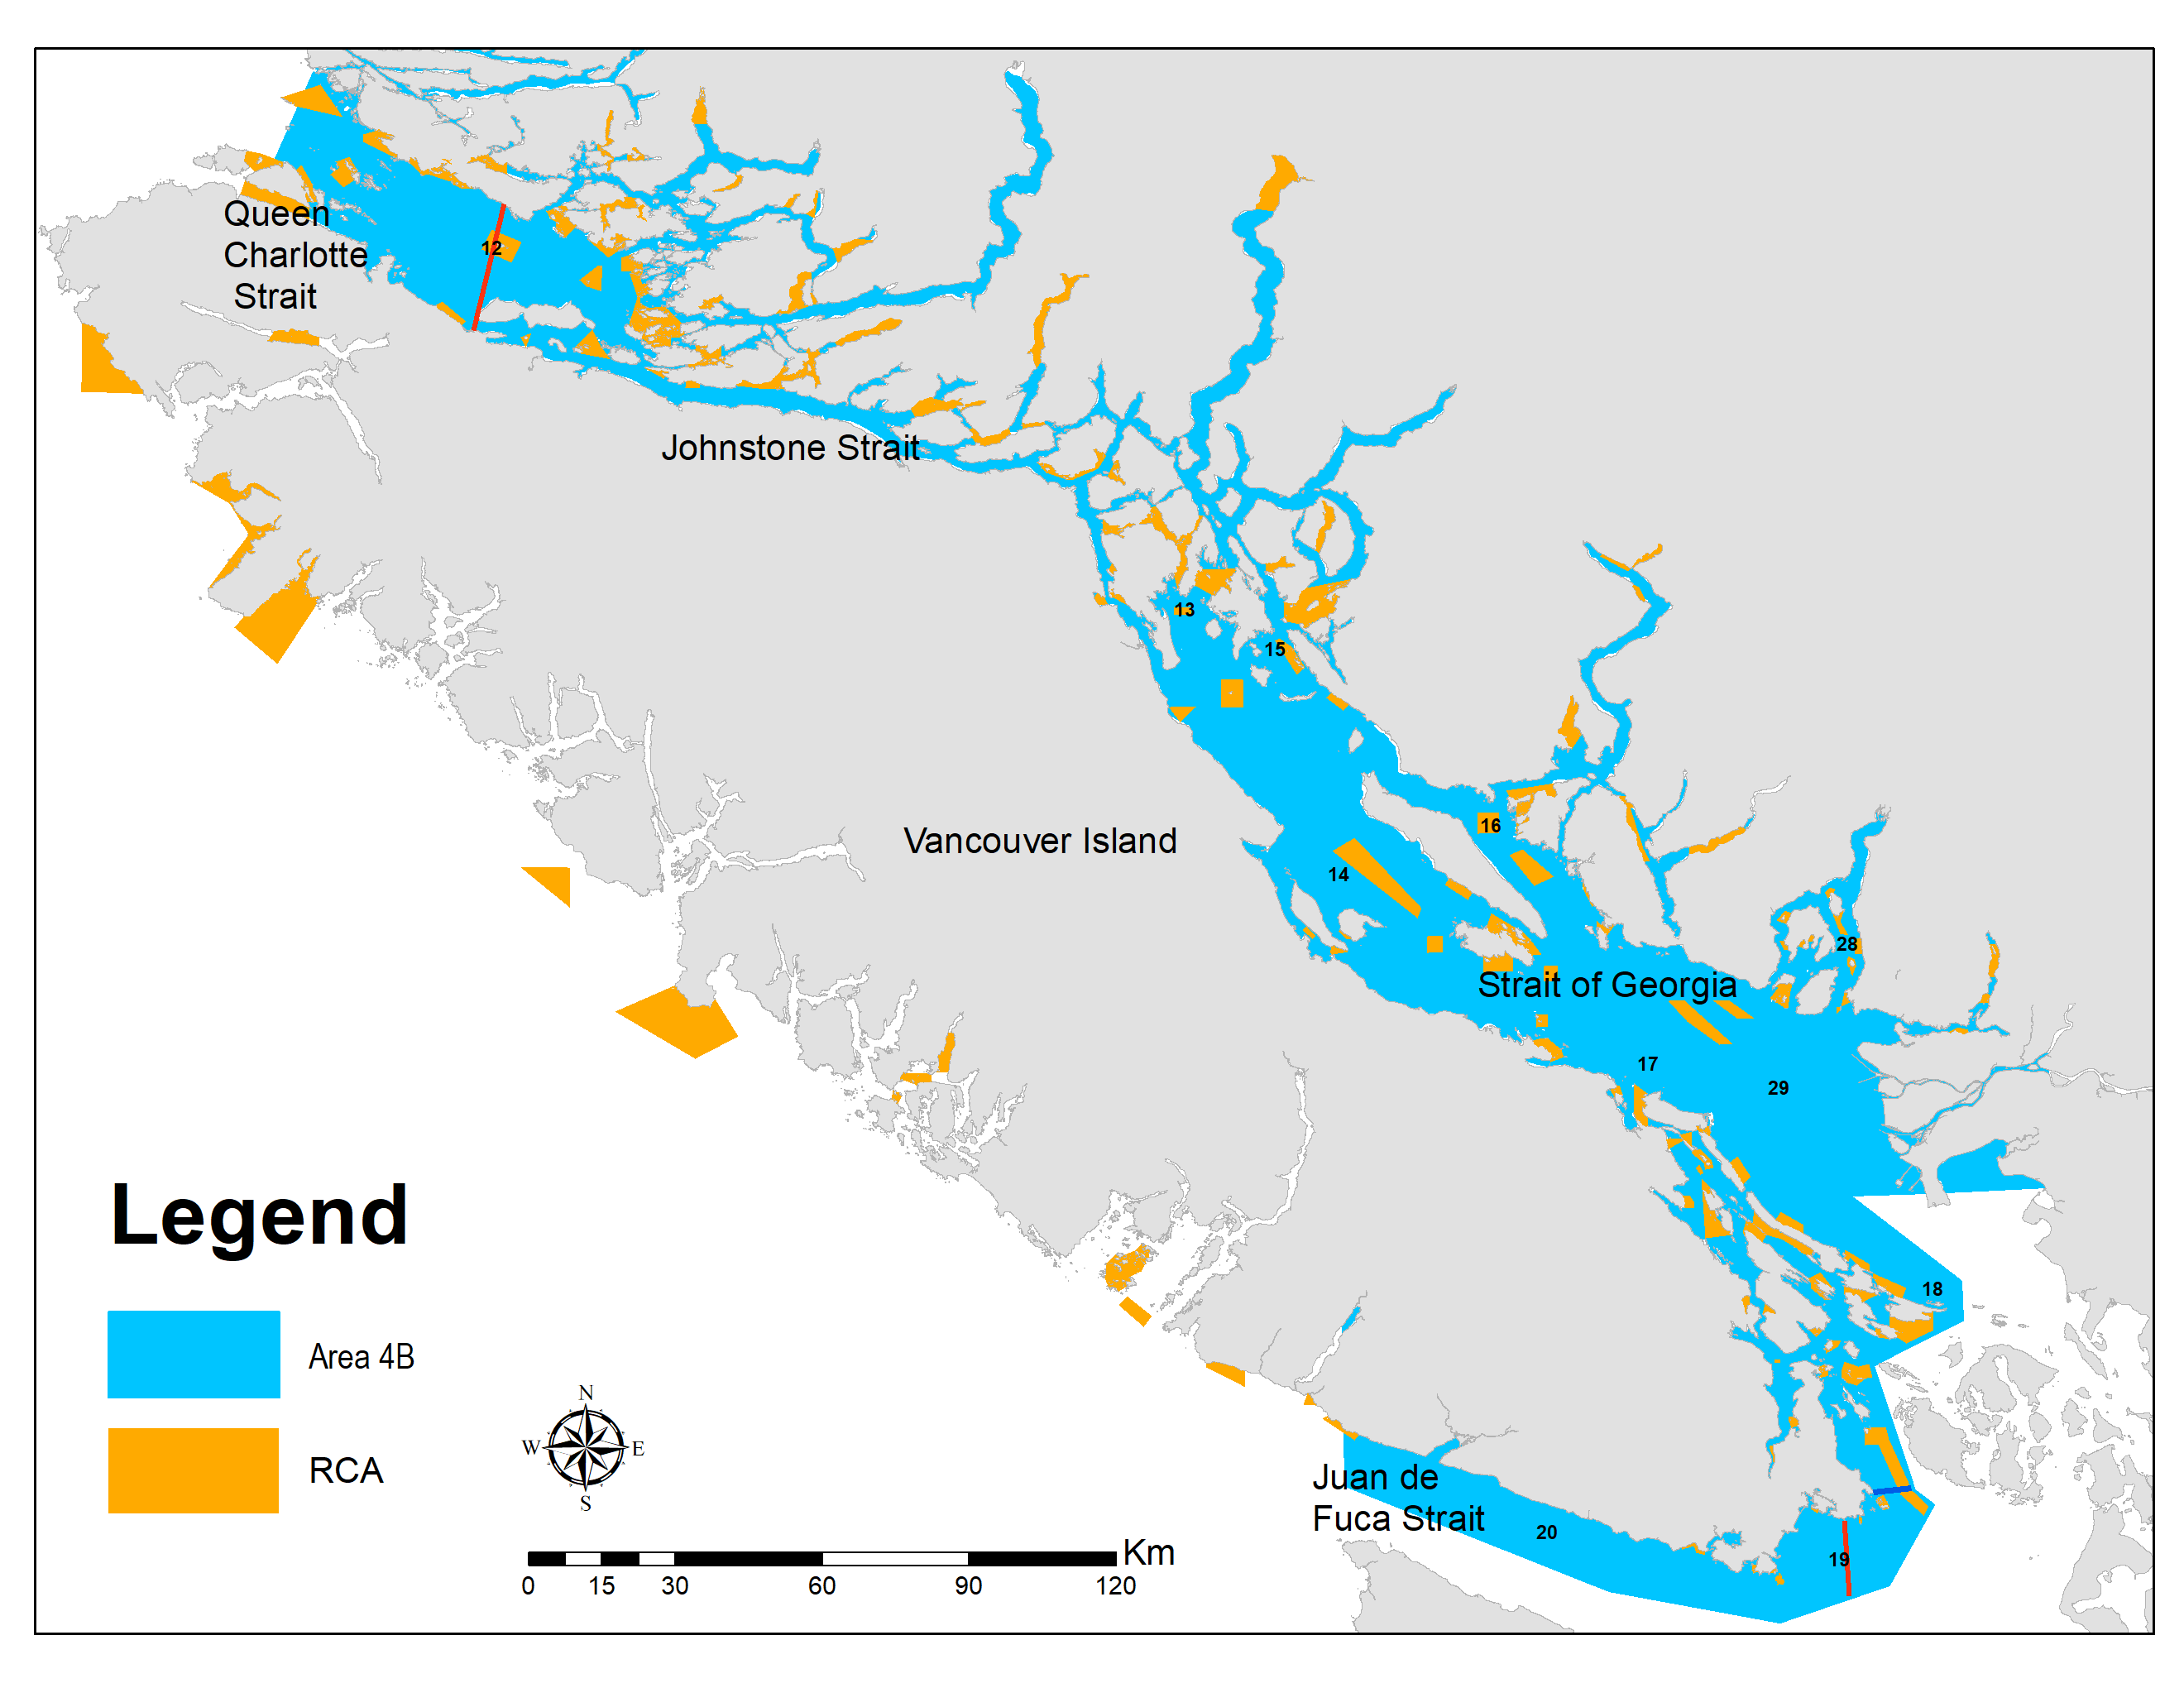
\includegraphics[width=5in]{C:/GitHub/yelloweye-inside/figs-french/InsideYE_Map_new}}{Figure \ref{fig:map-4B}} 

}

\caption{Carte de la zone de gestion 4B du poisson de fond montrant les aires de conservation du sébaste (ACS) et les limites séparant l'unité désignable (UD) du sébaste aux yeux jaunes des eaux intérieures de l'UD du sébaste aux yeux jaunes des eaux extérieures. Les lignes rouges indiquent une proposition d'ajustement de l'aire de répartition de l'UD des eaux intérieures, fondée sur des preuves génétiques récentes (Siegle \protect\hyperlink{ref-siegle2011}{2011}; Siegle et al. \protect\hyperlink{ref-siegle2013}{2013}; Andrews et al. \protect\hyperlink{ref-andrews2018}{2018}).}\label{fig:map-4B}
\end{figure}
L'objectif du plan de rétablissement actuel est de « reconstituer le stock au-dessus du PRL sur 80 ans avec une probabilité de réussite de 56 \% ». Le jalon cible est de « dégager des tendances positives au cours de chaque période de 10 ans ». La procédure de gestion actuelle du sébaste aux yeux jaunes des eaux intérieures vise à maintenir les prises annuelles totales (commerciales, récréatives, alimentaires, sociales et rituelles des Premières Nations et de relevé) à moins de 15 tonnes (voir l'annexe 9 du document DFO (\protect\hyperlink{ref-ifmp2018}{2018}) pour plus de renseignements).

D'après les directives, les plans de rétablissement au Canada doivent présenter une forte probabilité de rétablissement des stocks de poissons hors de la zone critique dans le délai prescrit (DFO \protect\hyperlink{ref-dfo2013}{2013}). Ce projet vise notamment à répondre à une préoccupation exprimée par les gestionnaires des pêches, à savoir que la probabilité de réussite de 56 \% énoncée dans le plan de rétablissement actuel (DFO \protect\hyperlink{ref-ifmp2018}{2018}) ne correspond pas à la définition d'une probabilité élevée.

Le document d'orientation indique également certaines mesures de gestion recommandées, comme le maintien des prélèvements par toutes les sources au niveau le plus bas possible, l'élaboration d'une règle de contrôle des prises et l'application de l'évaluation de la stratégie de gestion pour évaluer, par simulation, le rendement d'autres mesures de gestion pour atteindre les objectifs de rétablissement du stock (DFO \protect\hyperlink{ref-dfo2013}{2013}). Le plan de rétablissement actuel met en œuvre un total autorisé des captures annuel fixe de 15 tonnes (DFO \protect\hyperlink{ref-ifmp2018}{2018}), qui n'a pas été mis à l'essai par simulation.

Le sébaste aux yeux jaunes est une espèce qui vit longtemps (jusqu'à 121 ans en Colombie-Britannique, Keppel and Olsen \protect\hyperlink{ref-keppel2019}{2019}), dans des habitats démersaux rocheux répartis de manière irrégulière et discontinue sur la côte intérieure de la Colombie-Britannique (Yamanaka et al. \protect\hyperlink{ref-yamanaka2011}{2011}). Ces caractéristiques du cycle biologique rendent l'espèce vulnérable à la surexploitation par la pêche. Le stock des eaux intérieures est considéré comme étant à données limitées, car peu de données sont accessibles sur la composition selon l'âge, on manque de données biologiques sur les pêches commerciales, récréatives et des Premières Nations, et une incertitude entoure l'ampleur des prises historiques.

\hypertarget{sec:introduction-mse}{%
\subsection{ÉVALUATION DE LA STRATÉGIE DE GESTION}\label{sec:introduction-mse}}

À l'échelle mondiale, la fourniture d'avis scientifiques pour la gestion des pêches a évolué vers des approches axées sur l'évaluation de la stratégie de gestion (ou axées sur la gestion) (p.~ex., Butterworth and Punt \protect\hyperlink{ref-butterworth1999}{1999}; Rademeyer et al. \protect\hyperlink{ref-rademeyer2007}{2007}; Berkson and Thorson \protect\hyperlink{ref-berkson2015}{2015}; Geromont and Butterworth \protect\hyperlink{ref-geromont2015}{2015}; Carruthers et al. \protect\hyperlink{ref-carruthers2016}{2016}; Punt et al. \protect\hyperlink{ref-punt2016}{2016}). L'évaluation de la stratégie de gestion se concentre sur la détermination des procédures de gestion qui donnent les meilleurs résultats en ce qui concerne l'atteinte des objectifs convenus en matière de politique et de pêche, lorsqu'ils sont mis en œuvre dans un environnement de simulation en « boucle fermée » (figure~\ref{fig:mse-chart-basic}). Dans les pêches à production contrôlée, comme la pêche du poisson de fond en Colombie-Britannique, où les quotas sont gérés, les procédures de gestion décrivent les mesures de gestion pour l'établissement des limites des prises. Les données exigées dans les procédures de gestion peuvent varier considérablement, allant d'approches très riches en données, y compris les évaluations statistiques des prises selon l'âge avec des règles de contrôle des prises, à des règles de données simples (approches « limitées en données »), qui ne reposent que sur les données sur les prises et un indice de l'abondance (p.~ex., Geromont and Butterworth \protect\hyperlink{ref-geromont2015}{2015}; Carruthers et al. \protect\hyperlink{ref-carruthers2016}{2016}).

La simulation en boucle fermée diffère des approches d'évaluation classique des stocks parce qu'elle simule la rétroaction entre la mise en œuvre des procédures de gestion et le système sous-jacent (le stock de poisson et son environnement), décrite par un ou plusieurs modèles opérationnels. L'approche de la simulation en boucle fermée tient compte de l'effet des procédures de gestion sur le système, ainsi que des données futures recueillies dans le système et de leur utilisation chez les procédures de gestion (Punt et al. \protect\hyperlink{ref-punt2016}{2016}; Carruthers and Hordyk \protect\hyperlink{ref-carruthers2018}{2018}\protect\hyperlink{ref-carruthers2018}{a}; Anderson et al. \protect\hyperlink{ref-anderson2020gfmp}{2020}\protect\hyperlink{ref-anderson2020gfmp}{a}).


\begin{figure}[htb]

{\centering \pdftooltip{\includegraphics[width=6.3in]{C:/GitHub/yelloweye-inside/figs-french/mse-chart-simple2}}{Figure \ref{fig:mse-chart-basic}} 

}

\caption{Illustration du processus de simulation en boucle fermée des pêches d'après Anderson et al. (\protect\hyperlink{ref-anderson2020gfmp}{2020}\protect\hyperlink{ref-anderson2020gfmp}{a}), selon Punt et al. (\protect\hyperlink{ref-punt2016}{2016}). La procédure de gestion peut être fondée sur une règle de données simple (p.~ex., réduire les prises autorisées de x \% si l'indice du relevé diminue de y \%) ou peut être un modèle d'estimation combiné à une règle de contrôle des prises.}\label{fig:mse-chart-basic}
\end{figure}
\hypertarget{sec:introduction-approach}{%
\subsection{APPROCHE}\label{sec:introduction-approach}}

En raison des données limitées sur le stock de sébaste aux yeux jaunes des eaux intérieures, il est difficile d'évaluer le rendement prévu des mesures de gestion nécessaires pour rendre le stock conforme aux dispositions sur les stocks de poissons, c.-à-d.~pour le faire sortir de la zone critique dans le délai convenu et avec la probabilité convenue. La simulation-mise à l'essai en boucle fermée des procédures de gestion à données limitées permet d'évaluer le rendement relatif des procédures de gestion dans un éventail d'incertitudes entourant, par exemple, la biologie sous-jacente des poissons, l'erreur d'observation, l'erreur d'estimation et l'erreur de mise en œuvre (p.~ex., Kell et al. \protect\hyperlink{ref-kell2006}{2006}; Carruthers et al. \protect\hyperlink{ref-carruthers2016}{2016}).

Depuis 2017, une entente de partenariat entre l'Université de la Colombie-Britannique et le MPO (DFO \protect\hyperlink{ref-dfo_dlmtool_2017}{2017}) a facilité l'élaboration de deux progiciels à accès libre pour l'évaluation de la stratégie de gestion, mis en œuvre dans l'environnement de programmation statistique R (R Core Team \protect\hyperlink{ref-r2019}{2019})~: l'outil pour les méthodes à données limitées (DLMtool) (Carruthers and Hordyk \protect\hyperlink{ref-carruthers2018}{2018}\protect\hyperlink{ref-carruthers2018}{a}, \protect\hyperlink{ref-carruthers_hordyk_2018}{2018}\protect\hyperlink{ref-carruthers_hordyk_2018}{b}) et l'outil pour l'évaluation de la stratégie de gestion (MSEtool) (Huynh et al. \protect\hyperlink{ref-huynh_msetool_2019}{2019}). Après plusieurs années de développement, ces progiciels sont parmi les logiciels les plus rapides, les plus souples et les plus extensibles pour évaluer les stratégies de gestion des pêches. Ils peuvent être appliqués à des stocks pauvres ou riches en données, permettant d'évaluer rapidement plusieurs procédures de gestion en fonction d'objectifs de conservation et de pêche personnalisables, et d'évaluer les principaux compromis.

\hypertarget{sec:introduction-mp-framework}{%
\subsubsection{Cadre des procédures de gestion du poisson de fond en Colombie-Britannique}\label{sec:introduction-mp-framework}}

Le Cadre des procédures de gestion pour le poisson de fond en Colombie-Britannique (Anderson et al. \protect\hyperlink{ref-anderson2020gfmp}{2020}\protect\hyperlink{ref-anderson2020gfmp}{a}) a été élaboré parallèlement au présent document pour évaluer le rendement d'un large éventail de procédures de gestion pour les espèces de poisson de fond à données limitées. Le Cadre des procédures de gestion fait largement appel aux fonctions de DLMtool et de MSEtool, avec l'appui d'un progiciel R gfdlm (Anderson et al. \protect\hyperlink{ref-gfdlm}{2020}\protect\hyperlink{ref-gfdlm}{c}) rédigé par les auteurs de Anderson et al. (\protect\hyperlink{ref-anderson2020gfmp}{2020}\protect\hyperlink{ref-anderson2020gfmp}{a}), qui contient un ensemble d'outils de soutien logiciel et des visualisations personnalisées.

Nous suivons le Cadre des procédures de gestion pour sélectionner les procédures de gestion afin d'établir des limites des prises pour les stocks de poissons de fond à données limitées (Anderson et al. \protect\hyperlink{ref-anderson2020gfmp}{2020}\protect\hyperlink{ref-anderson2020gfmp}{a}). Notre évaluation du plan de rétablissement du sébaste aux yeux jaunes des eaux intérieures constitue la première application du Cadre des procédures de gestion pour produire un avis scientifique à l'appui des décisions sur les prises. Le cadre suit six étapes de pratiques exemplaires décrites ci-après et plus en détail dans Anderson et al. (\protect\hyperlink{ref-anderson2020gfmp}{2020}\protect\hyperlink{ref-anderson2020gfmp}{a}).

Les étapes des pratiques exemplaires sont fondées sur un examen effectué par Punt et al. (\protect\hyperlink{ref-punt2016}{2016}), qui a cerné cinq étapes clés du processus d'évaluation de la stratégie de gestion (étapes 2 à 6 ci-après). Une première étape supplémentaire du Cadre des procédures de gestion, qui définit le contexte décisionnel, a été définie par Gregory et al. (\protect\hyperlink{ref-gregory2012}{2012}) et Cox and Benson (\protect\hyperlink{ref-cox2016}{2016}). En grande partie, le logiciel DLMtool a été conçu pour permettre aux praticiens de suivre ces étapes (figure~\ref{fig:mse-chart}; Carruthers and Hordyk \protect\hyperlink{ref-carruthers2018}{2018}\protect\hyperlink{ref-carruthers2018}{a}).


\begin{figure}[htb]

{\centering \pdftooltip{\includegraphics[width=\textwidth]{C:/GitHub/yelloweye-inside/figs-french/mse-chart}}{Figure \ref{fig:mse-chart}} 

}

\caption{Les étapes du processus d'évaluation de la stratégie de gestion selon Punt et al. (\protect\hyperlink{ref-punt2016}{2016}), tel que mis en œuvre dans DLMtool. Copié de Anderson et al. (\protect\hyperlink{ref-anderson2020gfmp}{2020}\protect\hyperlink{ref-anderson2020gfmp}{a}) et adapté de Carruthers and Hordyk (\protect\hyperlink{ref-carruthers2018}{2018}\protect\hyperlink{ref-carruthers2018}{a}). Cette figure complète la figure~\ref{fig:mse-chart-basic}.}\label{fig:mse-chart}
\end{figure}
Les six étapes sont les suivantes~:

Étape 1~: Définition du contexte décisionnel.

Étape 2~: Choix des objectifs et des paramètres de rendement.

Étape 3~: Choix des incertitudes/spécification des modèles opérationnels.

Étape 4~: Détermination des procédures de gestion possibles.

Étape 5~: Simulation de l'application des procédures de gestion.

Étape 6~: Présentation des résultats et choix de la procédure de gestion.

Après la sélection et la mise en œuvre de la procédure de gestion pour l'établissement de la limite des prises (figure~\ref{fig:mse-chart}; par exemple, application de l'algorithme de la procédure de gestion sélectionnée à l'indice du relevé observé), la dernière étape nécessaire consiste à surveiller et à évaluer périodiquement le rendement de la procédure de gestion (DFO \protect\hyperlink{ref-dfo2013}{2013}; Dowling et al. \protect\hyperlink{ref-dowling2015a}{2015}; Carruthers and Hordyk \protect\hyperlink{ref-carruthers2018}{2018}\protect\hyperlink{ref-carruthers2018}{a}). Cela peut se faire par des moyens informels, comme à l'aide de la rétroaction des pêcheurs et des données des relevés (p.~ex., Cox and Kronlund \protect\hyperlink{ref-cox2008a}{2008}), ou au moyen de mesures statistiques plus formelles, où l'on compare les données observées aux prévisions des modèles opérationnels pour vérifier si le système fonctionne comme prévu (Butterworth \protect\hyperlink{ref-butterworth2008}{2008}; Carruthers and Hordyk \protect\hyperlink{ref-carruthers_hordyk_2018}{2018}\protect\hyperlink{ref-carruthers_hordyk_2018}{b}; discussion dans Anderson et al. \protect\hyperlink{ref-anderson2020gfmp}{2020}\protect\hyperlink{ref-anderson2020gfmp}{a}).

Dans les sections suivantes, nous décrivons notre approche pour l'élaboration d'un éventuel plan de rétablissement du sébaste aux yeux jaunes des eaux intérieures, en suivant les six étapes des pratiques exemplaires.

\hypertarget{sec:decision-context}{%
\section{DÉFINIR LE CONTEXTE DÉCISIONNEL}\label{sec:decision-context}}

Les principales questions qui guident la définition du contexte décisionnel de l'évaluation de la stratégie de gestion sont les suivantes~:
\begin{itemize}
\item
  Quelle est la décision exacte à prendre?
\item
  Quel est le délai pour prendre la décision?
\item
  Quels sont les rôles et responsabilités précis des parties concernées? Les parties sont les Sciences, la Gestion des pêches, les Premières Nations, l'industrie, le milieu universitaire et des organisations non gouvernementales.
\item
  Comment la décision finale sera-t-elle prise?
\end{itemize}
Pour ce plan de rétablissement, il faut décider de la procédure de gestion à utiliser pour déterminer les limites des prises pour la période allant jusqu'au prochain avis disponible sur les prises. Le Comité régional d'examen par les pairs devrait prendre la décision finale sur la procédure de gestion à appliquer pour déterminer les futures limites des prises sur une base consensuelle, après avoir examiné le contenu scientifique de l'avis (y compris la structure et le contenu des modèles opérationnels) et tenu compte du rendement relatif des procédures de gestion et des compromis entre les paramètres de rendement.

\#SÉLECTION DES OBJECTIFS ET DES PARAMÈTRES DE RENDEMENT \{\#sec:objectives-metrics\}

Il faut établir des objectifs clairs en matière de gestion et de pêche, ainsi que les paramètres de rendement qui permettent de les évaluer. Les objectifs peuvent couvrir un large éventail d'objectifs stratégiques ou législatifs (p.~ex., maintenir le stock au-dessus du PRL), d'objectifs économiques (p.~ex., maintenir des prises moyennes ou réduire la variabilité des prises) et d'objectifs culturels (p.~ex., maintenir l'accès minimal requis au stock ou à des zones de pêche particulières). Dans un scénario de rétablissement, les objectifs de conservation doivent avoir préséance. Cependant, dans un cadre de simulation, il est possible d'examiner des compromis entre la conservation et d'autres objectifs de pêche à court et à long terme, tant que l'objectif principal de conservation est atteint. Les objectifs entièrement quantifiés comprennent un paramètre ou une cible, la probabilité souhaitée de réussite et un délai pour atteindre l'objectif (p.~ex., la probabilité de maintenir le stock au-dessus du PRL est supérieure à 0,95 {[}19 fois sur 20{]} sur 1,5 génération du stock). Les paramètres de rendement sont des mesures quantifiées des objectifs. Dans une simulation en boucle fermée, ils sont calculés dans le modèle opérationnel à chaque étape temporelle des projections.

L'objectif initial du plan de rétablissement était de reconstituer le stock au-dessus du PRL sur 80 ans avec une probabilité de réussite de 56 \%. Un autre jalon cible était d'atteindre des tendances positives de la biomasse dans chaque période de 10 ans. La procédure de gestion convenue pour atteindre ces objectifs était de maintenir le TAC combiné (pêches commerciales, récréatives, ASR, de relevé biologique) à moins de 15 tonnes par année (DFO \protect\hyperlink{ref-ifmp2018}{2018}).

\hypertarget{sec:objectives-metrics-obj}{%
\subsection{OBJECTIFS ET JALONS}\label{sec:objectives-metrics-obj}}

Nous présentons un ensemble d'objectifs améliorés et les paramètres de rendement connexes pour le plan de rétablissement du sébaste aux yeux jaunes des eaux intérieures. Les principaux objectifs provisoires de conservation sont guidés par le Cadre de l'approche de précaution (DFO \protect\hyperlink{ref-dfo2006}{2006}, \protect\hyperlink{ref-dfo2009}{2009}), le document d'orientation du plan de rétablissement (DFO \protect\hyperlink{ref-dfo2013}{2013}) et les précédents régionaux (Cox et al. \protect\hyperlink{ref-cox2019}{2019}, \protect\hyperlink{ref-cox2020}{2020}). D'autres objectifs liés au rendement des pêches et à la variabilité du rendement annuel des pêches sont fondés sur des précédents dans d'autres analyses de la région du Pacifique du MPO (p.~ex., Cox and Kronlund \protect\hyperlink{ref-cox2008a}{2008}; Forrest et al. \protect\hyperlink{ref-forrest2018}{2018}; Cox et al. \protect\hyperlink{ref-cox2019}{2019}, \protect\hyperlink{ref-cox2020}{2020}).

L'objectif de conservation de base proposé est le suivant~:
\begin{enumerate}
\def\labelenumi{\arabic{enumi}.}

\item
  Ramener le stock au-dessus du PRL sur 56 ans (1,5 génération) avec une probabilité de réussite d'au moins 95 \% {[}19 fois sur 20{]}.
\end{enumerate}
Nous avons ajusté le délai de rétablissement initial de 80 ans (DFO \protect\hyperlink{ref-ifmp2018}{2018}) à 56 ans dans la présente analyse, en fonction de la durée de génération estimée pour le sébaste aux yeux jaunes des eaux extérieures (Cox et al. \protect\hyperlink{ref-cox2020}{2020}), en tenant compte de la directive selon laquelle le rétablissement doit être réalisé dans un délai de 1,5 à 2 durées de génération (DFO \protect\hyperlink{ref-dfo2013}{2013}). Pour de plus amples renseignements sur la durée de génération, consulter l'annexe~\ref{app:biological-data}, section~\ref{sec:generation}. Nous avons fait passer la probabilité de réussite souhaitée de 56 \% à 95 \% pour tenir compte de la directive selon laquelle la probabilité de rétablissement doit être élevée, ainsi que des pratiques exemplaires internationales, où les politiques de nombreuses administrations visent à maintenir les stocks au-dessus du PRL avec une probabilité de 90 \% à 95 \% {[}18 à 19 fois sur 20{]} (Sainsbury \protect\hyperlink{ref-sainsbury2008}{2008}; McIlgorm \protect\hyperlink{ref-mcilgorm2013}{2013}).

Nous proposons également les objectifs supplémentaires suivants, précisés dans la section~\ref{sec:objectives-metrics-pm}:
\begin{enumerate}
\def\labelenumi{\arabic{enumi}.}
\setcounter{enumi}{1}
\item
  Reconstituer le stock au-dessus du RSS sur 56 ans (1,5 génération).
\item
  Reconstituer le stock au-dessus du PRL sur 38 ans (1 génération).
\item
  Les objectifs de conservation ci-dessus étant atteints, maintenir des prises cibles moyennes à court et à long terme.
\item
  Les objectifs de conservation ci-dessus étant atteints, réduire au minimum la variabilité des prises dans les pêches d'une année à l'autre.
\end{enumerate}
Il convient de noter que nous n'avons pas attribué de probabilités cibles à ces objectifs, car elles sont fournies aux fins de l'évaluation des compromis avec l'objectif 1. Toutefois, nous avons éliminé les procédures de gestion qui ne respectaient pas la probabilité minimale de maintenir les prises au-dessus de 10 tonnes à court terme (voir la section~\ref{sec:simulation}).

En plus des objectifs susmentionnés, nous proposons de peaufiner les jalons définis dans le plan de rétablissement initial (DFO \protect\hyperlink{ref-ifmp2018}{2018}) en ajoutant le texte en italiques comme suit~:
\begin{enumerate}
\def\labelenumi{\arabic{enumi}.}
\setcounter{enumi}{5}

\item
  Atteindre des tendances positives de la biomasse dans chaque période de 10 ans \emph{tant que le stock demeure inférieur au PRL}.
\end{enumerate}
La période de 10 ans indiquée dans les jalons du plan de rétablissement actuel du sébaste aux yeux jaunes des eaux intérieures (DFO \protect\hyperlink{ref-ifmp2018}{2018}) reflétait une hypothèse selon laquelle le rétablissement hors de la zone critique pourrait être très lent pour ce stock. Nous avons ajusté le jalon pour tenir compte de l'hypothèse selon laquelle, une fois que le stock n'est plus dans la zone critique, le jalon ne sera plus nécessaire. La directive actuelle sur le rétablissement (DFO \protect\hyperlink{ref-dfo2013}{2013}) ne prévoit que des objectifs pour faire sortir les stocks de la zone critique, avec des jalons visant à garantir que les progrès sont réalisés pendant le processus de rétablissement. Elle mentionne des objectifs à plus long terme pour poursuivre le rétablissement des stocks jusque dans la zone saine, au-dessus du RSS. Toutefois, cela est censé se produire après la période du plan de rétablissement et en dehors de la portée de ce dernier (DFO \protect\hyperlink{ref-dfo2013}{2013}).

\hypertarget{sec:objectives-metrics-pm}{%
\subsection{PARAMÈTRES DE RENDEMENT}\label{sec:objectives-metrics-pm}}

Nous proposons les paramètres de rendement suivants pour mesurer les objectifs, où \emph{B} représente la biomasse féconde, RMD le rendement maximal durable, \emph{B}\textsubscript{RMD} la biomasse féconde à l'équilibre au rendement maximal durable, DG représente la durée d'une génération, et EAMP l'écart absolu moyen des prises (\(C\)) sur les \(n\) années (remarque~: \emph{CT} = court terme, \emph{LT} = long terme). Nous définissons le PRL et le RSS comme 0,4\emph{B}\textsubscript{RMD} et 0,8\emph{B}\textsubscript{RMD}, respectivement, en suivant les définitions provisoires du Cadre de l'approche de précaution (DFO \protect\hyperlink{ref-dfo2006}{2006}), utilisées dans l'évaluation des stocks de 2010 (Yamanaka et al. \protect\hyperlink{ref-yamanaka2011}{2011}). Dans les simulations en boucle fermée, tous les points de référence et les paramètres de rendement sont calculés dans le modèle opérationnel. Les paramètres de rendement bruts sont calculés pour chacune des 100 années de la période de projection et résumés en fonction de la période d'intérêt~: 1. \textbf{PRL 1,5DG}~: P(\emph{B} \textgreater{} 0,4 \emph{B}\textsubscript{RMD}) après 1,5 DG (en 2075, année 56 de la période de projection) 2. \textbf{RSS 1,5DG}~: P(\emph{B} \textgreater{} 0,8 \emph{B}\textsubscript{RMD}) après 1,5 DG (en 2075, année 56 de la période de projection) 3. \textbf{PRL 1DG}~: P(\emph{B} \textgreater{} 0,4 \emph{B}\textsubscript{RMD}) après 1 DG (en 2057, année 38 de la période de projection) 4. \textbf{CT C10}~: P(prises moyennes \textgreater{} 10 tonnes) de 2020 à 2029, années 1 à 10 de la période de projection 5. \textbf{CT C15}~: P(prises moyennes \textgreater{} 15 tonnes) de 2020 à 2029, années 1 à 10 de la période de projection 6. \textbf{LT C20}~: P(prises moyennes \textgreater{} 20 tonnes) après 1 DG (en 2057, année 38 de la période de projection) 7. \textbf{CT EAMP}~: P(EAMP\textsubscript{2020-2029} \textless{} EAMP\textsubscript{2012-2019})

Nous avons inclus le paramètre de rendement PRL 1 DG pour nous assurer que les procédures de gestion ne mènent pas le stock à l'effondrement à court terme. Nous avons choisi 10 tonnes, 15 tonnes et 20 tonnes comme cibles de prises, qui représentent des niveaux de prises de 5 tonnes inférieurs et supérieurs au TAC actuel de 15 tonnes.

Nous avons calculé EAMP\textsubscript{2020-2029} comme suit~:
\begin{equation}
\textrm{AADC}_\textrm{2020-2029} = \dfrac{1}{9}\sum_{y=2021}^{2029} \mid C_y - C_{y-1} \mid.
\end{equation}
Une période de référence (de 2012 à 2019) a été choisie, car elle marque le début du TAC de 15 tonnes. Nous avons calculé EAMP\textsubscript{2012-2019} comme suit~:
\begin{equation}
\textrm{AADC}_\textrm{2012-2019} = \dfrac{1}{7}\sum_{y=2013}^{2019} \mid C_y - C_{y-1} \mid.
\end{equation}
Lorsque les paramètres de rendement sont calculés sur plusieurs années, il faut prendre soin d'expliquer clairement la façon dont les statistiques sommaires sont calculées. Anderson et al. (\protect\hyperlink{ref-anderson2020gfmp}{2020}\protect\hyperlink{ref-anderson2020gfmp}{a}) suggéraient provisoirement de calculer les statistiques de rendement sur les répétitions et les années pour toute la période définie pour le paramètre de rendement. Nous suivons ce protocole. Par exemple, nous avons calculé la moyenne des paramètres des prises à court terme par rapport aux répétitions et aux années 2020 à 2029.

\hypertarget{sec:om}{%
\section{CHOIX DES INCERTITUDES/SPÉCIFICATION DES MODÈLES OPÉRATIONNELS}\label{sec:om}}

Les modèles opérationnels de l'outil DLMtool sont organisés en quatre composantes principales représentant un réseau hydrographique exploité réel~:
\begin{enumerate}
\def\labelenumi{\arabic{enumi}.}

\item
  la dynamique des populations du stock de poissons (p.~ex., croissance, recrutement, mortalité);
\item
  la dynamique de la pêche (p.~ex., sélectivité, ciblage spatial);
\item
  les processus d'observation (p.~ex., biais et précision des indices des relevés);
\item
  la mise en œuvre de la gestion (p.~ex., dépassement des limites de prises).
\end{enumerate}
Les équations et les paramètres décrivant les quatre composantes des modèles opérationnels sont fournis en détail à l'annexe B de Carruthers and Hordyk (\protect\hyperlink{ref-carruthers2018}{2018}\protect\hyperlink{ref-carruthers2018}{a}) et à l'annexe A de Anderson et al. (\protect\hyperlink{ref-anderson2020gfmp}{2020}\protect\hyperlink{ref-anderson2020gfmp}{a}). L'outil DLMtool permet d'intégrer l'incertitude dans de nombreux paramètres des modèles opérationnels grâce à la spécification facultative des distributions de probabilité. Afin d'isoler davantage les effets de certaines sources d'incertitude sur le rendement des procédures de gestion, nous élaborons d'autres modèles opérationnels qui modifient la valeur (ou la distribution) d'un ou de plusieurs paramètres ou sources de données d'intérêt (section~\ref{sec:approach3-oms}).

La pratique exemplaire recommande d'étalonner ou de conditionner les modèles opérationnels à l'aide des données observées, afin qu'ils puissent reproduire les observations historiques. Le progiciel complémentaire de DLMtool, MSEtool (Huynh et al. \protect\hyperlink{ref-huynh_msetool_2019}{2019}), comprend une mise en œuvre efficace d'une analyse de réduction du stock (Kimura and Tagart \protect\hyperlink{ref-kimura1982}{1982}; Walters et al. \protect\hyperlink{ref-walters2006}{2006}), qui est en fait un modèle statistique des prises selon l'âge qui estime les combinaisons historiques de la mortalité par pêche et du recrutement qui correspondraient aux données observées. L'analyse de réduction du stock est décrite en détail à l'annexe B de Anderson et al. (\protect\hyperlink{ref-anderson2020gfmp}{2020}\protect\hyperlink{ref-anderson2020gfmp}{a}).

Le cadre de simulation comporte deux périodes distinctes~: 1) la période historique, qui comprend toutes les années, de la première année de la série chronologique des prises observées \(t_1\) à la dernière année de cette série chronologique \(t_c\) (où « c » représente l'année « en cours »); 2) la période de projection, qui va de la première année suivant \(t_c\) à la dernière année de la projection \(t_N\). La période historique est conditionnée par des observations historiques à l'aide de l'analyse de réduction du stock (voir l'annexe B dans Anderson et al. \protect\hyperlink{ref-anderson2020gfmp}{2020}\protect\hyperlink{ref-anderson2020gfmp}{a}). Les simulations en boucle fermée, avec application des procédures de gestion et calcul des paramètres de rendement, commencent la première année de la période de projection (année \(t_{c+1}\)).

L'élaboration d'un modèle opérationnel dans le cadre des procédures de gestion comporte trois étapes.
\begin{enumerate}
\def\labelenumi{\arabic{enumi}.}
\item
  Définir les valeurs et les plages des paramètres dans le modèle opérationnel.
\item
  Envoyer les paramètres du modèle opérationnel dans le modèle d'analyse de réduction du stock, qui conditionne le modèle opérationnel en l'ajustant aux prises observées historiques, aux indices de l'abondance et à toutes les données accessibles sur la composition selon l'âge. On obtient des estimations conditionnées des paramètres du modèle et des estimations de la biomasse historique et de la mortalité historique par pêche (les années \(t_1\) à \(t_c\)), qui sont conformes aux observations historiques.
\item
  Renvoyer les valeurs des paramètres conditionnés au modèle opérationnel (maintenant le modèle opérationnel « conditionné ») pour les utiliser dans les projections de simulation en boucle fermée, à partir de l'année \(t_{c+1}\).
\end{enumerate}
Dans la mesure du possible, nous avons dérivé les paramètres du modèle opérationnel à partir de toutes les données biologiques accessibles des relevés dans la zone 4B, qui sont principalement recueillies dans le cadre des relevés à la palangre sur fond dur dans les eaux intérieures (annexe~\ref{app:biological-data}). Nous avons tiré d'autres paramètres de la documentation scientifique et des évaluations des stocks de sébaste aux yeux jaunes dans d'autres régions (voir les renseignements détaillés dans l'annexe~\ref{app:desc-om-yelloweye}). Une liste des réglages « par défaut » des paramètres du modèle opérationnel recommandés pour la plupart des stocks de poisson de fond de la Colombie-Britannique est fournie à l'annexe C de Anderson et al. (\protect\hyperlink{ref-anderson2020gfmp}{2020}\protect\hyperlink{ref-anderson2020gfmp}{a}).

Nous avons conditionné les modèles opérationnels avec l'analyse de réduction du stock, en utilisant les données sur la composition selon l'âge provenant des relevés de recherche (annexe~\ref{app:biological-data}), les indices des relevés à la palangre sur fond dur dans les eaux intérieures (annexe~\ref{app:index-data}) et les données sur les prises des pêches commerciales et récréatives (annexe~\ref{app:catch-data}). Les résultats du conditionnement des modèles opérationnels sont fournis ci-après dans la section~\ref{sec:approach3-conditioning}.

\hypertarget{sec:approach3-oms}{%
\subsection{MODÈLES OPÉRATIONNELS}\label{sec:approach3-oms}}

La pratique exemplaire en matière d'évaluation de la stratégie de gestion recommande de diviser les essais en un « ensemble de référence » de modèles opérationnels de base, qui comprend les incertitudes les plus importantes (p.~ex., épuisement du stock ou plage des valeurs de la mortalité naturelle) et un « ensemble de robustesse », afin de refléter un plus grand éventail d'incertitudes peut-être moins plausibles, mais qu'il est néanmoins intéressant d'explorer (Rademeyer et al. \protect\hyperlink{ref-rademeyer2007}{2007}). Anderson et al. (\protect\hyperlink{ref-anderson2020gfmp}{2020}\protect\hyperlink{ref-anderson2020gfmp}{a}) recommandent de présenter séparément les paramètres de rendement des ensembles de référence et de robustesse. Ils préconisent, pour la plupart des résultats, de calculer la moyenne des paramètres de rendement de l'ensemble de référence pour tous les scénarios de l'ensemble de référence de modèles opérationnels (une approche d'ensemble à intégrer pour toutes les incertitudes du modèle opérationnel), mais de présenter séparément les paramètres de rendement des différents scénarios de l'ensemble de robustesse de modèles opérationnels. La présentation distincte des résultats de l'ensemble de robustesse permet aux gestionnaires de voir comment les procédures de gestion qui ont donné de bons résultats dans l'ensemble de référence se comportent pour un ensemble d'hypothèses plus diversifiées (Rademeyer et al. \protect\hyperlink{ref-rademeyer2007}{2007}).

Pour le sébaste aux yeux jaunes des eaux intérieures, nous avons établi quatre modèles opérationnels de l'ensemble de référence~: (1) un modèle opérationnel de référence; (2) un modèle opérationnel reflétant une autre hypothèse au sujet de l'ampleur des prises historiques entre 1986 et 2005; (3) un modèle opérationnel prévoyant des événements de recrutement futurs épisodiques (rares, mais importants); (4) un modèle opérationnel estimant la sélectivité dans le relevé à la palangre sur fond dur (tableau~\ref{tab:ye-scen}).

Nous avons également établi deux modèles opérationnels de l'ensemble de robustesse englobant d'autres sources d'incertitude~: (A) un modèle opérationnel qui suppose une mortalité naturelle plus faible que les autres modèles opérationnels; (B) un modèle opérationnel qui suppose un coefficient de variation (CV) plus élevé dans le futur relevé à la palangre sur fond dur (tableau~\ref{tab:ye-scen}).
\begin{longtable}[]{@{}ll@{}}
\caption{\label{tab:ye-scen}Scénarios de modèle opérationnel pour le sébaste aux yeux jaunes des eaux intérieures..}\tabularnewline
\toprule
Nom du scénario de modèle opérationnel & Type d'ensemble\tabularnewline
\midrule
\endfirsthead
\toprule
Nom du scénario de modèle opérationnel & Type d'ensemble\tabularnewline
\midrule
\endhead
(1) Base & Reference\tabularnewline
(2) Low catch & Reference\tabularnewline
(3) Episodic recruitment & Reference\tabularnewline
(4) Estimate HBLL selectivity & Reference\tabularnewline
(A) Low M & Robustness\tabularnewline
(B) High HBLL CV & Robustness\tabularnewline
\bottomrule
\end{longtable}
\hypertarget{sec:approach3-reference}{%
\subsubsection{Reference set}\label{sec:approach3-reference}}

The following OMs were developed as the reference set. We hereafter refer to them by their numbers, e.g., OM Scenario (1).

\hypertarget{sec:approach3-reference1}{%
\subsubsection{(1) Base}\label{sec:approach3-reference1}}

Data sources are provided in Appendices~\ref{app:biological-data} through~\ref{app:catch-data}. Parameter settings for the Base OM are provided in Appendix~\ref{app:desc-om-yelloweye}. We here provide a brief description of the Base OM assumptions that were adjusted in other OM scenarios.

There are two main uncertainties associated with the historical commercial catch time series for Inside Yelloweye Rockfish (details in Appendix~\ref{app:catch-data}, Section~\ref{sec:com-catch-data}). These are: (1) aggregated reporting of rockfish as Other Rockfish (ORF; rockfish species other than Pacific Ocean Perch) and (2) the magnitude of unreported catch that was discarded at sea prior to the introduction of 100\% at-sea monitoring in the groundfish longline fleet in 2006 (Stanley et al. \protect\hyperlink{ref-stanley2009}{2009}). For consistency with Yamanaka et al. (\protect\hyperlink{ref-yamanaka2011}{2011}), we doubled the nominal catch data for the period 1986---2005, as industry did not have confidence in the catch data for those years {[}DFO (\protect\hyperlink{ref-dfo2012}{2012}); see Appendix~\ref{app:catch-data}, Section~\ref{sec:com-catch-data}{]}.

Projected recruitment deviations were sampled in log space with standard deviation \(\tau = 0.4\), with autocorrelation estimated post-hoc from the historical recruitment deviates in the SRA model (Appendix A of Anderson et al. \protect\hyperlink{ref-anderson2020gfmp}{2020}\protect\hyperlink{ref-anderson2020gfmp}{a}).

The Inside Yelloweye Rockfish stock is indexed by two fishery-independent surveys: the inside Hard Bottom Longline Survey (Appendix~\ref{app:index-data}, Section~\ref{sec:hbll-index-data}) and the Dogfish Survey (Appendix~\ref{app:index-data}, Section~\ref{sec:dogfish-index-data}). The SRA model exhibited better retrospective behaviour when the SRA model was fit with more likelihood weight applied to the Dogfish Survey. The age of full selectivity in the HBLL survey was fixed at 22 years (see Section~\ref{sec:approach3-conditioning} below).

Historical commerical CPUE was also available and used as an index of abundance for conditioning the OM (Yamanaka et al. \protect\hyperlink{ref-yamanaka2011}{2011}). Following the decisions made for the 2011 assessment, the time series was divided into three stanzas (1986-1990, 1995-2001, and 2003-2005), representing periods when fishery behaviour is likely to have changed in response to management regulations (Appendix~\ref{app:catch-data}, Section~\ref{sec:management-changes}).

Natural mortality (\emph{M}) was sampled from a probability distribution based on that used by Yamanaka et al. (\protect\hyperlink{ref-yamanaka2011}{2011}), where \(M \sim \textrm{Lognormal}(0.045, 0.2)\) (Appendix~\ref{app:desc-om-yelloweye}, Section~\ref{app:desc-stock-m-yelloweye}).

During the projection period, only the HBLL index was assumed to be available for the MPs, as this survey is conducted annually. Projecting only one index of abundance is consistent with many data-limited MPs, which only use a single index of abundance (see Appendix~\ref{app:mps}). Observation error in the projected index values was simulated with random deviates from a lognormal distribution with mean of 1 and standard deviation of 0.25 based on the estimated observation error in the HBLL index.

All other OM scenarios were adjusted from this baseline OM and differed only in terms of adjustments to key parameters or data sources, described below.

\hypertarget{sec:approach3-reference2}{%
\subsubsection{(2) Low catch}\label{sec:approach3-reference2}}

In the ``Low catch'' OM scenario, we test model sensitivity to the assumption of large unreported catch for the period 1986--2005. Instead of doubling nominal catch data for this period, the SRA was fit to the nominal catch data. As for the other OM scenarios, we used the reconstructed catch up to 1985 and the nominal catch from 1986 onwards.

\hypertarget{sec:approach3-reference3}{%
\subsubsection{(3) Episodic recruitment}\label{sec:approach3-reference3}}

Long-lived, late-maturing species such as Pacific rockfishes often exhibit episodic, or periodic, recruitment strategies characterized by high fecundity and occasional very large recruitment events (Winemiller and Rose \protect\hyperlink{ref-winemiller1992}{1992}; Rose et al. \protect\hyperlink{ref-rose2001}{2001}; Winemiller \protect\hyperlink{ref-winemiller2005}{2005}). This life history strategy is sometimes called the storage effect (Warner and Chesson (\protect\hyperlink{ref-warner1985}{1985})) because strong recruitment events are stored in the adult population and are capable of contributing to reproduction, sometimes significantly, when favourable conditions return. Longevity in rockfish is thought to have evolved as a strategy for weathering un-favourable conditions. Very large or even extreme year classes have been observed for several BC rockfish species (e.g., Pacific Ocean Perch: Haigh et al. \protect\hyperlink{ref-haigh2019}{2019}; Bocaccio: Haigh and Starr \protect\hyperlink{ref-haigh2020}{2020}).

To address the possibility that future recruitment during the projection period could be characterized by occasional very large recruitment events, we included an ``Episodic recruitment'' OM scenario. This OM scenario addresses the concern that very large cohorts are not adequately modelled by the lognormal distribution for recruitment deviations that was used in OM Scenario (1). In the Episodic recruitment OM scenario, recruitment deviations \(\varepsilon_{R,y}\) for each year of the projection period are generated as:
\begin{equation}
\varepsilon_{R,y} = 
\left\{
\begin{array}{ll}
\varepsilon^{(1)}_{R,y} & \eta_y = 0\\
\varepsilon^{(3)}_{R,y} & \eta_y = 1,
\end{array}
\right.
\end{equation}
where \(\varepsilon^{(1)}_{R,y}\) is the recruitment deviation from OM Scenario (1) and \(\log\varepsilon^{(3)}_{R,y} \sim \textrm{Normal}(-0.5\tau^2, \tau)\) represents the ``episodic'' recruitment distribution with \(\tau = 2\) (standard deviation). The parameter \(\eta_y\) is a Bernoulli random variable \(\eta_y \sim \textrm{Bernoulli}(p = 1/38)\), which selects whether an extreme recruitment event will occur. We assume that an extreme recruitment event is expected to occur once every generation (38 years), based on the observation that strong recruitment events in Inside Yelloweye Rockfish were present in 1948 and 1970. Although recent environmental conditions may be favourable for some species of rockfishes (Haigh and Starr \protect\hyperlink{ref-haigh2020}{2020}; Lincandeo et al. \protect\hyperlink{ref-lincandeo2020}{2020}), we don't yet have any evidence of recent strong recruitment events for Inside Yelloweye Rockfish that might indicate more frequent episodic or spasmodic recruitment events.

\hypertarget{sec:approach3-reference4}{%
\subsubsection{(4) Estimate HBLL selectivity}\label{sec:approach3-reference4}}

Annual sample sizes of age-composition data from research surveys are very small (Appendix~\ref{app:biological-data}). This makes estimation of selectivity in the surveys highly uncertain, which led to the choice to fix survey selectivity in the other OM scenarios.

Given large uncertainty in our choice of selectivity, we allowed the SRA to estimate selectivity for the surveys in this OM scenario and utilized the available survey age-composition data.

\hypertarget{sec:approach3-robustness}{%
\subsubsection{Robustness set}\label{sec:approach3-robustness}}

The following OMs were developed as the robustness set. We hereafter refer to them by their letters.

\hypertarget{sec:approach3-referenceA}{%
\subsubsection{(A) Low M}\label{sec:approach3-referenceA}}

Lower values of natural mortality have been used for Inside Yelloweye Rockfish (Yamanaka and Lacko \protect\hyperlink{ref-yamanaka2001}{2001}; COSEWIC \protect\hyperlink{ref-cosewic2008}{2008}; Wood et al. \protect\hyperlink{ref-wood2019}{2019}). This OM scenario used a lower mean in the distribution for \emph{M}, with \(M \sim \textrm{Lognormal}(0.025, 0.2)\), reflecting the possibility that the stock could be less productive than assumed in the other OM scenarios.

\hypertarget{sec:approach3-referenceB}{%
\subsubsection{(B) Higher HBLL CV}\label{sec:approach3-referenceB}}

This OM scenario considers the possibility that the future HBLL index might be less precise than assumed in the other OM scenarios. Instead of an observation standard deviation \(\sigma_I = 0.25\), we use the standard deviation (\(\sigma_I\)) and autocorrelation (\(\theta_\textrm{AC}\)) from the index residuals in OM Scenario (1), obtained from the SRA fit to the HBLL index.

This \(\sigma_I\) has a mean of 0.41 and a range of 0.38--0.44.

\hypertarget{sec:approach3-conditioning}{%
\subsection{CONDITIONING THE OPERATING MODELS}\label{sec:approach3-conditioning}}

After specifying the OM parameters (Appendix~\ref{app:desc-om-yelloweye}), we conditioned the OMs using the SRA model described in Appendix B of Anderson et al. (\protect\hyperlink{ref-anderson2020gfmp}{2020}\protect\hyperlink{ref-anderson2020gfmp}{a}).

Note that the DLMtool OM combines all fleets into a single fleet. However, if the OM is conditioned using the SRA model, the SRA can accommodate multiple fleets, and selectivity is fleet-specific. In this case, fishery selectivity in the OM for the projection period is replaced with the SRA-conditioned estimates of fishing mortality-at-age in the final year of the historical period (\(t_c\)), normalized by dividing by apical fishing mortality in that year. This essentially provides the DLMtool OM with relative selectivity-at-age, weighted by catch across all fleets. The closed-loop simulation projections therefore assume that the relative selectivity across fleets remains constant in the projection period.

Similarly, if the OM is conditioned using the SRA model, analysts can also specify (or estimate) selectivity parameters for the individual indices of abundance (in this case two fishery-independent surveys and three commercial CPUE series (Figure~\ref{fig:survey-fits})). In this case, the SRA passes all of the indices back to DLMtool, preserving the estimated or user-defined selectivities-at-age for each index. However, note that the DLMtool MPs only utilize a single index of abundance (see Appendix~\ref{app:mps}). In the current study, all index-based MPs utilize the inside HBLL survey.

We used the SRA to populate the following parameters in the conditioned OMs:
\begin{itemize}

\item
  \(B_{t_c}/B_0\) (or ``D''; depletion in the last historical year \(t_c\))
\item
  \(R_0\) (unfished recruitment)
\item
  \(\theta_\textrm{AC}\) (or ``AC''; first-order autocorrelation of recruitment deviations)
\item
  \(\varepsilon_{\textrm{R},y}\) for years \(t_1\) to \(t_c\) (annual recruitment deviations)
\item
  \(F_{a,y}\) (fishing mortality at age by year)
\end{itemize}
See Appendix B of Anderson et al. (\protect\hyperlink{ref-anderson2020gfmp}{2020}\protect\hyperlink{ref-anderson2020gfmp}{a}) for details on these parameters.

The SRA was run for 250 replicates. Each replicate used a different value of \emph{M} and \emph{h} (sampled independently from the distributions shown in Appendix~\ref{app:desc-om-yelloweye}, except for OM Scenario (A), which used a different distribution for \emph{M}). The model was initialized under the assumption that spawning biomass (\(B_y\)) was in an unfished equilibrium state prior to 1918, the first year of the time series, i.e., \(B_{1918} = B_0\). While this is unlikely to be true, as First Nations and others would have been catching Yelloweye Rockfish prior to 1918, these numbers are expected to be small enough not to impact the outcomes of the performance of MPs in the projection period.

\hypertarget{sec:approach3-conditioning-base-om}{%
\subsubsection{Selection of base OM}\label{sec:approach3-conditioning-base-om}}

Initial attempts to fit the SRA model did not produce good fits to the dogfish survey. Furthermore, retrospective analysis showed persistent retrospective bias in annual estimates of spawning biomass when sequentially removing 11 years of data (when evaluated at the mean values of \emph{M} and \emph{h}, Figure~\ref{fig:retro-initial}, top panel). The choice to base retrospective analysis on 11 years of data was primarily to evaluate sensitivity of the model to removal of each year of data, going back to 2009, the terminal year for the 2011 assessment.

Increasing the likelihood weight for the SRA fit to the Dogfish survey (\(\lambda^I_s = 4\); Equation B.22 in Anderson et al. \protect\hyperlink{ref-anderson2020gfmp}{2020}\protect\hyperlink{ref-anderson2020gfmp}{a}), and fixing age-at-full-selectivity in the HBLL survey to 22 years, removed the retrospective pattern (Figure~\ref{fig:retro-initial}, bottom panel). Therefore, for OM Scenario (1) and all other OM scenarios except Scenario (4), we fixed the age-at-full selectivity of the HBLL Survey at 22 years (Figure~\ref{fig:HBLL-selectivity}), while also upweighting the Dogfish survey.


\begin{figure}[htb]

{\centering \pdftooltip{\includegraphics[width=4.25in]{C:/GitHub/yelloweye-inside/mse/figures/retrospective-spawning-biomass}}{Figure \ref{fig:retro-initial}} 

}

\caption{Retrospective patterns in spawning biomass for the initial fit and OM Scenario (1). Coloured lines represent estimates of spawning biomass with \(X\) years of data removed, where \(X\) is shown in the legend for each series.}\label{fig:retro-initial}
\end{figure}
There are a number of factors that increase uncertainty in estimating selectivity for the Dogfish survey e.g.~the absence of biological data from this survey, and changes in fishing operations and hook type that occurred in 2004 (Appendix~\ref{app:index-data}, Section~\ref{sec:dogfish-index-data}). There are also several differences between the HBLL and Dogfish longline surveys (Appendix~\ref{app:index-data}, Section~\ref{sec:dogfish-index-data}), but, for the reasons mentioned, we cannot reliably estimate the selectivity for the Dogfish survey. Out of necessity, selectivity in the Dogfish survey was set to mirror selectivity in the HBLL survey, whether it was estimated (OM Scenario (4)) or fixed (all other OM scenarios).

Age composition data from the commerical fishery were available from a single fishing trip in 1989, and length samples from 2002--2019 were identified from the recreational fishery. Attempts to fit the SRA model to these data did not produce satisfactory estimates of selectivity. The estimated values of the age of full selectivity were very high, suggesting that most ages were not completely vulnerable to the fishery, and significantly differed from values estimated for the Outside Yelloweye population (Cox et al. \protect\hyperlink{ref-cox2020}{2020}). Since it is unlikely that selectivity varies to such an extent between geographical regions, these data were not further considered.

As a result, selectivity for these gears was fixed in all OM scenarios (Figure~\ref{fig:sra-selectivity}). Parameter values were set so that the selectivity-at-age curves approximated those estimated by Cox et al. (\protect\hyperlink{ref-cox2020}{2020}) for the commercial longline and recreational fisheries for outside Yelloweye Rockfish (see Appendix~\ref{app:desc-om-yelloweye}, Section~\ref{app:desc-fleet-selectivity-yelloweye}). As noted above, these selectivities were returned to the DLMtool OMs as a combined-fleet selectivity curve from the terminal year (\(t_c\)) of the historical period (Figure~\ref{fig:om-selectivity}).

\hypertarget{sec:approach3-conditioning-results}{%
\subsubsection{OM conditioning results}\label{sec:approach3-conditioning-results}}

The following sections describe the results of conditioning the OMs.

\hypertarget{sec:approach3-conditioning-indices}{%
\subsubsection{Fits to data}\label{sec:approach3-conditioning-indices}}

The predicted catch in the SRA models matched the catch data by design, which was achieved by setting the standard deviation of the observation error to a value of 0.01 (Anderson et al. \protect\hyperlink{ref-anderson2020gfmp}{2020}\protect\hyperlink{ref-anderson2020gfmp}{a}, their Equation B.27).

The SRA was able to fit to the indices of abundance reasonably well (Figure~\ref{fig:survey-fits}) and convergence was achieved for all replicates in all OM scenarios. For all OM scenarios, the estimated index fell within the observed confidence intervals in most years, although there were some outliers (Figure~\ref{fig:survey-fits}). The fit to the early 1986 and 1989 observations in the Dogfish Survey was slightly better in OM Scenario (A), which is consistent with a less productive, more depleted stock. However, these two observations are more uncertain than those in recent years, due to changes in fishing operations and hook type that occurred in 2004 (Appendix~\ref{app:index-data}, Section~\ref{sec:dogfish-index-data}). Fits to the commercial CPUE series were generally good, due to the short time stanzas for each series (Figure~\ref{fig:survey-fits}).


\begin{figure}[htb]

{\centering \pdftooltip{\includegraphics[width=\textwidth]{C:/GitHub/yelloweye-inside/mse/figures/ye-index-fits}}{Figure \ref{fig:survey-fits}} 

}

\caption{SRA model fits to the HBLL, Dogfish, and three commercial CPUE relative indices. Panels from left to right represent OM scenarios. Thin lines represent individual SRA model fits across stochastic draws from the various OM parameters. Dots represent index mean and line segments represent 2 times the standard errors as entered into the SRA models.}\label{fig:survey-fits}
\end{figure}
The SRA model fit the survey age-composition data reasonably well, despite very small sample sizes (Figures~\ref{fig:sra-conditioned-comp-fit1} to~\ref{fig:sra-conditioned-comp-fitB}). We note that in comparing OM Scenarios (1) and (4) it appears that fixing or estimating selectivity in the HBLL survey did not generate very different fits to the age composition data (Figures~\ref{fig:sra-conditioned-comp-fit1} and~\ref{fig:sra-conditioned-comp-fit4}).

For most years, the SRA predicted larger abundance in the plus group (80+ \emph{y}) than what was observed. A lack of fish older than 80 \emph{y} in the survey suggested that total mortality could have been greater in the past than estimated in our OMs. This could be represented in the OMs in two ways. First, \emph{M} could be increased in the models. However, our preliminary model investigations indicated that increasing \emph{M} also increases retrospective bias. Secondly, the catch history could be changed to predict higher values of fishing mortality. This was done in OM Scenario (2) by assuming lower catches in 1986-2005, which resulted in a slightly smaller stock (Figure~\ref{fig:biomass-om}) and higher fishing mortality (Figure~\ref{fig:F-om}). However, the estimated plus group was only slightly reduced in most years for this OM scenario (Figure~\ref{fig:sra-conditioned-comp-fit2}).

This issue is a challenge for very long-lived species with poor age-composition sampling. With such small sample sizes, there is a relatively small chance of observing very old fish. Large structural uncertainties in the model and available data (e.g., the Dogfish survey, catch data) made it difficult to resolve one issue, e.g., persistent overprediction of old fish, without generating another issue, e.g., retrospective bias.

\clearpage


\begin{figure}[htb]

{\centering \pdftooltip{\includegraphics[width=0.85\textwidth]{C:/GitHub/yelloweye-inside/mse/figures/conditioning/HBLL_age_comp_updog_fixsel}}{Figure \ref{fig:sra-conditioned-comp-fit1}} 

}

\caption{SRA model fits to the survey age composition data for OM Scenario (1), showing observed (points) and estimated (green lines) proportions. Sample sizes (N) are number of sets from which age samples were collected in each year.}\label{fig:sra-conditioned-comp-fit1}
\end{figure}
\clearpage


\begin{figure}[htb]

{\centering \pdftooltip{\includegraphics[width=0.85\textwidth]{C:/GitHub/yelloweye-inside/mse/figures/conditioning/HBLL_age_comp_lowcatch_fixsel}}{Figure \ref{fig:sra-conditioned-comp-fit2}} 

}

\caption{SRA model fits to the survey age composition data for OM Scenario (2), showing observed (points) and estimated (green lines) proportions. Sample sizes (N) are number of sets from which age samples were collected in each year.}\label{fig:sra-conditioned-comp-fit2}
\end{figure}
\clearpage


\begin{figure}[htb]

{\centering \pdftooltip{\includegraphics[width=0.85\textwidth]{C:/GitHub/yelloweye-inside/mse/figures/conditioning/HBLL_age_comp_episodic_recruitment}}{Figure \ref{fig:sra-conditioned-comp-fit3}} 

}

\caption{SRA model fits to the survey age composition data for OM Scenario (3), showing observed (points) and estimated (green lines) proportions. Sample sizes (N) are number of sets from which age samples were collected in each year.}\label{fig:sra-conditioned-comp-fit3}
\end{figure}
\clearpage


\begin{figure}[htb]

{\centering \pdftooltip{\includegraphics[width=0.85\textwidth]{C:/GitHub/yelloweye-inside/mse/figures/conditioning/HBLL_age_comp_upweight_dogfish}}{Figure \ref{fig:sra-conditioned-comp-fit4}} 

}

\caption{SRA model fits to the survey age composition data for OM Scenario (4), showing observed (points) and estimated (green lines) proportions. Sample sizes (N) are number of sets from which age samples were collected in each year.}\label{fig:sra-conditioned-comp-fit4}
\end{figure}
\clearpage


\begin{figure}[htb]

{\centering \pdftooltip{\includegraphics[width=0.85\textwidth]{C:/GitHub/yelloweye-inside/mse/figures/conditioning/HBLL_age_comp_lowM_fixsel}}{Figure \ref{fig:sra-conditioned-comp-fitA}} 

}

\caption{SRA model fits to the survey age composition data for OM Scenario (A), showing observed (points) and estimated (green lines) proportions. Sample sizes (N) are number of sets from which age samples were collected in each year.}\label{fig:sra-conditioned-comp-fitA}
\end{figure}
\clearpage


\begin{figure}[htb]

{\centering \pdftooltip{\includegraphics[width=0.85\textwidth]{C:/GitHub/yelloweye-inside/mse/figures/conditioning/HBLL_age_comp_high_index_cv}}{Figure \ref{fig:sra-conditioned-comp-fitB}} 

}

\caption{SRA model fits to the survey age composition data for OM Scenario (B), showing observed (points) and estimated (green lines) proportions. Sample sizes (N) are number of sets from which age samples were collected in each year.}\label{fig:sra-conditioned-comp-fitB}
\end{figure}
\hypertarget{sec:approach3-conditioning-parameters}{%
\subsubsection{Parameter estimates}\label{sec:approach3-conditioning-parameters}}

The OM reference and robustness scenarios rendered a range of estimated parameter values (Figure~\ref{fig:sra-conditioned-parameters}).


\begin{figure}[htb]

{\centering \pdftooltip{\includegraphics[width=0.85\textwidth]{C:/GitHub/yelloweye-inside/mse/figures/ye-sra-estimated}}{Figure \ref{fig:sra-conditioned-parameters}} 

}

\caption{Histograms of parameters estimated by the SRA. AC refers to \(\theta_\textrm{AC}\). D refers to depletion (\(B_{t_c}/B_0\)). For visualization purposes, the \emph{R}\textsubscript{0} axis limits have been restricted to a maximum of 490 and the AC axis limits to a minimum of 0.76. This excludes a small number of replicates.}\label{fig:sra-conditioned-parameters}
\end{figure}
Estimated means and coefficients of variation (CV) for reference points \emph{F}\textsubscript{MSY}, \emph{B}\textsubscript{MSY} and MSY are provided in Table~\ref{tab:sra-ref-pts}. The CVs are large due to the large range of sampled values for \emph{M} and \emph{h} (Appendix~\ref{app:desc-om-yelloweye}, Sections~\ref{app:desc-stock-m-yelloweye} and~\ref{app:desc-stock-h-yelloweye}).
\begin{longtable}[]{@{}llll@{}}
\caption{\label{tab:sra-ref-pts}Estimated reference points for each OM Scenario. Standard deviations across replicates are shown in parentheses.}\tabularnewline
\toprule
OM Scenario & F\textsubscript{MSY} (/y) & B\textsubscript{MSY} (t) & MSY (t)\tabularnewline
\midrule
\endfirsthead
\toprule
OM Scenario & F\textsubscript{MSY} (/y) & B\textsubscript{MSY} (t) & MSY (t)\tabularnewline
\midrule
\endhead
(1) Base & 0.04 (0.33) & 1362.08 (0.27) & 63.92 (0.64)\tabularnewline
(2) Low catch & 0.04 (0.33) & 1087.02 (0.55) & 53.01 (1.12)\tabularnewline
(3) Episodic recruitment & 0.04 (0.33) & 1362.08 (0.27) & 63.92 (0.64)\tabularnewline
(4) Estimate HBLL selectivity & 0.04 (0.33) & 1199.70 (0.18) & 54.75 (0.44)\tabularnewline
(A) Low M & 0.02 (0.29) & 1384.54 (0.11) & 34.30 (0.20)\tabularnewline
(B) High HBLL CV & 0.04 (0.33) & 1362.08 (0.27) & 63.92 (0.64)\tabularnewline
\bottomrule
\end{longtable}
\clearpage

\hypertarget{sec:approach3-conditioning-trajectories}{%
\subsubsection{Historical trajectories}\label{sec:approach3-conditioning-trajectories}}

In all OM scenarios, except OM Scenario (A), the median spawning biomass in 2019 is estimated to be above the LRP (Figure~\ref{fig:biomass-om}). OM Scenario (A) estimated median spawning biomass to have been below the LRP for most years after 2000 and less than 50\% probability of being above the LRP in 2019 (Figure~\ref{fig:ref-pt}). OM Scenario (2) and OM Scenario (4) also had a small probability of being below the LRP in the current year. Therefore, according to all the reference set OM scenarios and one robustness set OM scenario, the stock can already be considered to have rebuilt above the LRP. The median spawning biomass is estimated to be above the USR in OM Scenarios (1), (2), (3), and (B); and estimated to be below the USR in OM Scenarios (4) and (A).

All OM scenarios predicted a slight increase in spawning biomass during the last decade of the time series (Figure~\ref{fig:biomass-om}). The credible interval for all OM scenarios except (A) was very broad, arising from uncertainties in natural mortality and steepness (Figure~\ref{fig:sra-conditioned-parameters}). Note that trajectories are identical for OM Scenarios (1), (3) and (B), as OM Scenarios (3) and (B) only differ from OM Scenario (1) in the treatment of parameters in the projection period. The very narrow credible interval for OM Scenario (A) reflects the very low fixed value of \emph{M} in this OM scenario, restricting the range of possible outcomes.

The implied spawning biomass depletion trajectories during the historical period from the eight OMs follow the same pattern as those for \emph{B} (Figure~\ref{fig:depletion-om}).

Estimates of historical recruitment deviations were similar across OM scenarios (Figure~\ref{fig:recdev-om}).

Estimated historical apical fishing mortality varied across OM scenarios, with larger values estimated for OM Scenarios (4) and (A), the more depleted trajectories (Figure~\ref{fig:F-om}). All OM scenarios predicted large peaks in fishing mortality during the 1980s and 1990s (Figure~\ref{fig:F-om}).


\begin{figure}[htb]

{\centering \pdftooltip{\includegraphics[width=\textwidth]{C:/GitHub/yelloweye-inside/mse/figures/ye-compare-SRA-MSY-panel}}{Figure \ref{fig:biomass-om}} 

}

\caption{Spawning biomass relative to spawning biomass at MSY (\emph{B}/\emph{B}\textsubscript{MSY}) trajectories for reference and robustness set OMs. Lines represent medians, and dark and light grey shading represent 50\% and 95\% quantiles across replicates, respectively. Dotted horizontal lines represent the USR (0.8 \emph{B}\textsubscript{MSY}) and LRP (0.4 \emph{B}\textsubscript{MSY}).}\label{fig:biomass-om}
\end{figure}

\begin{figure}[htb]

{\centering \pdftooltip{\includegraphics[width=2.5in]{C:/GitHub/yelloweye-inside/mse/figures/historical_indicators_ref_pt}}{Figure \ref{fig:ref-pt}} 

}

\caption{Probability that the 2019 spawning biomass is above the LRP and USR for the six operating models.}\label{fig:ref-pt}
\end{figure}

\begin{figure}[htb]

{\centering \pdftooltip{\includegraphics[width=\textwidth]{C:/GitHub/yelloweye-inside/mse/figures/ye-compare-SRA-depletion-panel}}{Figure \ref{fig:depletion-om}} 

}

\caption{Spawning biomass depletion trajectories for reference and robustness set OMs. Depletion is represented as a fraction of \(B_0\) (spawning biomass at unfished equilibrium). Lines represent individual replicates.}\label{fig:depletion-om}
\end{figure}

\begin{figure}[htb]

{\centering \pdftooltip{\includegraphics[width=\textwidth]{C:/GitHub/yelloweye-inside/mse/figures/ye-compare-SRA-recdev-panel}}{Figure \ref{fig:recdev-om}} 

}

\caption{Historical recruitment deviations estimated by the SRA model (in log space). Lines represent individual replicates.}\label{fig:recdev-om}
\end{figure}

\begin{figure}[htb]

{\centering \pdftooltip{\includegraphics[width=\textwidth]{C:/GitHub/yelloweye-inside/mse/figures/ye-compare-SRA-F-panel}}{Figure \ref{fig:F-om}} 

}

\caption{Apical fishing mortality (\(F_y\)) trajectories for reference and robustness set OMs. Apical fishing mortality is the maximum \(F_y\) experienced by fish of any age in a given year. Lines represent individual replicates.}\label{fig:F-om}
\end{figure}
\clearpage

\hypertarget{surplus-production-model-om-scenario}{%
\subsection{SURPLUS PRODUCTION MODEL OM SCENARIO}\label{surplus-production-model-om-scenario}}

The 2011 stock assessment for Inside Yelloweye Rockfish applied a Bayesian state space surplus production (SP) model, fit to catch, commercial CPUE, and the HBLL and Dogfish surveys (Yamanaka et al. \protect\hyperlink{ref-yamanaka2011}{2011}). The assessment estimated a 90\% {[}nine times out of 10{]} probability that the stock was below the LRP, i.e., in the critical zone. The assessment results triggered a rebuilding plan (DFO \protect\hyperlink{ref-ifmp2018}{2018}), which is updated in this document. The SRA models under all OM scenarios in the current analysis predict similar biomass trajectories to that in Yamanaka et al. (\protect\hyperlink{ref-yamanaka2011}{2011}). However, only OM Scenario (A) estimates the stock to have been below the LRP during the 2000s (Figure~\ref{fig:biomass-om}).

Model results diverged between the two analyses due to large differences in model structure between the SP model used in Yamanaka et al. (\protect\hyperlink{ref-yamanaka2011}{2011}) and the SRA used here. To explore the effects of model structure on stock status, we fit a SP model to the currently-available catch, CPUE and fishery-independent indices of abundance. We used the SP model implemented in the R software package MSEtool (Huynh et al. \protect\hyperlink{ref-huynh_msetool_2019}{2019}), fully described in Appendix D of Anderson et al. (\protect\hyperlink{ref-anderson2020gfmp}{2020}\protect\hyperlink{ref-anderson2020gfmp}{a}), which was configured to resemble the 2011 assessment as much as possible, although the model used here estimated parameters using maximum likelihood. The SP model set \emph{B}\textsubscript{MSY} to 50\% of unfished biomass, set the initial biomass in 1918 to 90\% of unfished biomass, and used a prior probability distribution for the intrinsic rate of population growth (\emph{r}) as a likelihood penalty. The prior probability distribution for \emph{r} was normally distributed with a mean of 0.068 and standard deviation of 0.03, based on values used in Yamanaka et al. (\protect\hyperlink{ref-yamanaka2011}{2011}).

SP model results more closely matched those of the previous assessment, estimating the stock to be below the LRP (Figure~\ref{fig:spm-biomass}). The model estimated the reference points \emph{B}\textsubscript{MSY} = 1844 t, \emph{F}\textsubscript{MSY} = 0.03 \emph{y}\textsuperscript{-1}, and MSY = 62 t. MSY and \emph{F}\textsubscript{MSY} estimates were similar to those from the SRA Base OM (Table~\ref{tab:sra-ref-pts}), but the estimate of \emph{B}\textsubscript{MSY} was approximately 35\% higher for the SP model than the SRA. We note that very similar findings were made by Cox et al. (\protect\hyperlink{ref-cox2020}{2020}) in the rebuilding plan for the outside stock of Yelloweye Rockfish. Their analysis, also based on age-structured models, predicted the current stock status for Outside Yelloweye Rockfish to be above the LRP, i.e., not in need of rebuilding, in contrast to results obtained by the SP model used in the 2014 stock assessment (Yamanaka et al. \protect\hyperlink{ref-yamanaka2018yelloweyeoutside}{2018}).

Notably, the biomass trends for the inside population since 2000 also differs between the two types of models. A flat, stable trend (below the LRP) was estimated in the SP model. On the other hand, many of the OMs developed from the SRA indicated that stock size has been increasing, although the trend is much flatter in the Low M scenario. We attempted four alternative model fits in an attempt to find scenarios that would mirror the biomass trend estimated in the SP model (Figure~\ref{fig:alt-SRA-fit}).

First, the dogfish survey was further downweighted with a likelihood weighting factor \(\lambda = 0.1\). This did not change the spawning biomass trend and the resulting stock status was more optimistic compared to the Base OM. Second, the 2019 dogfish survey value was excluded from the likelihood since the observed mean is higher than in previous recent years (with \(\lambda = 4\) following the Base OM). This scenario also did not appreciably affect the spawning biomass trend and magnitude. Third, the survey age comps was downweighted with \(\lambda = 0.1\). Similar to the first alternative, the spawning biomass trend was similar to the Base OM although the resultant stock status was somewhat less optimistic. Finally, the survey age comps were removed from the likelihood with \(\lambda = 0\). This scenario estimated the stock to be below the LRP in concordance with the SP model.

These results suggest that differences in estimated stock status between the current analysis and the previous stock assessment (Yamanaka et al. \protect\hyperlink{ref-yamanaka2011}{2011}) are in large part due to the data types included in the respective models and model structure. Both use catch and indices of abundance although the SP model leaves out the age compositions. When the two models use the same data types, i.e., excluding the age compositions from the likelihood with fixed assumptions regarding survey selectivity, both behave more similarly.

The age-structured model was chosen over the SP model to develop operating models for inside yelloweye rockfish on first principles. The age-structured model is more realistic in modeling delays in stock productivity over time. A single cohort contributes to the spawning biomass (and vulnerable biomass) over several years as it progresses through the age structure of the population. This mechanism can explain the increasing biomass estimated in the SRA. As fishing mortality decreased from catch reductions in the late 1990s into 2000, the spawning biomass started to increase. Also, the age of 5\% maturity is lower than the age of 5\% selectivity of the commercial fleet which would allow portions of cohorts to spawn before significant vulnerability to fishing.

For the SP model, this delay may be implicitly incorporated in the production function of the SP model but the biomass predicted in a given year is explicitly a function of the biomass observed in the previous year. Furthermore, the stock biomass in the SP model is implicitly vulnerable biomass since there are no explicit assumptions about selectivity. There is more difficulty in explaining the productivity of the stock mechanistically as all biological processes regarding growth, natural mortality, and maturity is incorporated in the intrinsic rate parameter \emph{r}.


\begin{figure}[htb]

{\centering \pdftooltip{\includegraphics[width=0.8\textwidth]{C:/GitHub/yelloweye-inside/mse/figures/SP_fit}}{Figure \ref{fig:spm-biomass}} 

}

\caption{Biomass relative to biomass at MSY (\emph{B}/\emph{B}\textsubscript{MSY}) trajectory from the SP model. Dotted horizontal lines represent the USR (0.8 \emph{B}\textsubscript{MSY}) and LRP (0.4 \emph{B}\textsubscript{MSY}).}\label{fig:spm-biomass}
\end{figure}

\begin{figure}[htb]

{\centering \pdftooltip{\includegraphics[width=5.5in]{C:/GitHub/yelloweye-inside/mse/figures/alt_SRA_fit}}{Figure \ref{fig:alt-SRA-fit}} 

}

\caption{Relative spawning biomass (\emph{B}/\emph{B}\textsubscript{MSY}) from alternative fits to the SRA that downweighted or eliminated data from the likelihood. Mean values of natural mortality and steepness were used. Dotted horizontal lines represent the USR (0.8 \emph{B}\textsubscript{MSY}) and LRP (0.4 \emph{B}\textsubscript{MSY}). The Base and Exclude 2019 dogfish scenarios overlap and the corresponding lines are jittered in the figure for clarity.}\label{fig:alt-SRA-fit}
\end{figure}
\clearpage

\hypertarget{computational-environment}{%
\section{COMPUTATIONAL ENVIRONMENT}\label{computational-environment}}

This version of the document was generated on 2021-05-31 11:03:06 with R version 3.6.3 (2020-02-29) (R Core Team \protect\hyperlink{ref-r2019}{2019}) and R package versions:
\begin{longtable}[]{@{}lll@{}}
\toprule
Package & Version & Date\tabularnewline
\midrule
\endhead
bookdown & 0.17 & 2020-01-11\tabularnewline
cowplot & 1.0.0 & 2019-07-11\tabularnewline
csasdown & 0.0.10.9000 & 2021-05-25\tabularnewline
DLMtool & 5.4.1 & 2019-12-06\tabularnewline
dplyr & 0.8.4 & 2020-01-31\tabularnewline
gfdata & 0.0.0.9000 & 2020-03-04\tabularnewline
gfdlm & 0.0.1.9000 & 2020-03-26\tabularnewline
gfplot & 0.1.4 & 2019-12-10\tabularnewline
ggplot2 & 3.2.1 & 2019-08-10\tabularnewline
knitr & 1.28 & 2020-02-06\tabularnewline
MSEtool & 1.4.3 & 2020-01-10\tabularnewline
purrr & 0.3.3 & 2019-10-18\tabularnewline
rmarkdown & 2.1 & 2020-01-20\tabularnewline
tidyr & 1.0.2 & 2020-01-24\tabularnewline
TMB & 1.7.16 & 2020-01-15\tabularnewline
\bottomrule
\end{longtable}
The source code for this document is available at:\\
\url{https://github.com/pbs-assess/yelloweye-inside/tree/2f9a8a4}.

This document was compiled with the R package csasdown (Anderson et al. \protect\hyperlink{ref-csasdown}{2020}\protect\hyperlink{ref-csasdown}{b}).

The specific versions of the primary packages used to generate this report can be viewed at:

\url{https://github.com/DLMtool/DLMtool/tree/fa971cf}\\
\url{https://github.com/tcarruth/MSEtool/tree/fa1498c}~\\
\url{https://github.com/pbs-assess/gfdata/tree/7292039}~\\
\url{https://github.com/pbs-assess/gfplot/tree/e0b36c0}~\\
\url{https://github.com/pbs-assess/gfdlm/tree/b895686}~\\
\url{https://github.com/pbs-assess/csasdown/tree/f9d5081}~\\

\vspace{4mm}

or installed via:

\texttt{\#\ install.packages(\textquotesingle{}devtools\textquotesingle{})}\\
\texttt{devtools::install\_github(\textquotesingle{}DLMtool/DLMtool\textquotesingle{},\ ref\ =\ \textquotesingle{}fa971cf\textquotesingle{})}~\\
\texttt{devtools::install\_github(\textquotesingle{}tcarruth/MSEtool\textquotesingle{},\ ref\ =\ \textquotesingle{}fa1498c\textquotesingle{})}~\\
\texttt{devtools::install\_github(\textquotesingle{}pbs-assess/gfdata\textquotesingle{},\ ref\ =\ \textquotesingle{}7292039\textquotesingle{})}~\\
\texttt{devtools::install\_github(\textquotesingle{}pbs-assess/sha\_gfplot\textquotesingle{},\ ref\ =\ \textquotesingle{}e0b36c0\textquotesingle{})}~\\
\texttt{devtools::install\_github(\textquotesingle{}pbs-assess/gfdlm\textquotesingle{},\ ref\ =\ \textquotesingle{}b895686\textquotesingle{})}~\\
\texttt{devtools::install\_github(\textquotesingle{}pbs-assess/csasdown\textquotesingle{},\ ref\ =\ \textquotesingle{}f9d5081\textquotesingle{})}~\\

\clearpage

\hypertarget{refs}{}
\leavevmode\hypertarget{ref-anderson2020gfmp}{}%
Anderson, S.C., Forrest, R.E., Huynh, Q.C., and Keppel, E.A. 2020a. A management procedure framework for groundfish in British Columbia. DFO Can. Sci. Advis. Sec. Res. Doc. 2020/nnn: In prep.

\leavevmode\hypertarget{ref-csasdown}{}%
Anderson, S.C., Grandin, C., Edwards, A.M., Grinnell, M.H., Ricard, D., and Haigh, R. 2020b. csasdown: Reproducible CSAS reports with bookdown. R package version 0.0.8. \url{https://github.com/pbs-assess/csasdown}.

\leavevmode\hypertarget{ref-gfdlm}{}%
Anderson, S.C., Grandin, C., and Forrest, R.E. 2020c. gfdlm: Tools for working with DLMtool and MSEtool. R package version 0.0.1.9000. \url{https://github.com/pbs-assess/gfdlm}.

\leavevmode\hypertarget{ref-andrews2018}{}%
Andrews, K.S., Nichols, K.M., Elz, A., Tolimieri, N., Harvey, C.J., Pacunski, R., Lowry, D., Yamanaka, K.L., and Tonnes, D.M. 2018. Cooperative research sheds light on population structure and listing status of threatened and endangered rockfish species. Conserv. Genet. 19(4): 865--878.

\leavevmode\hypertarget{ref-berkson2015}{}%
Berkson, J., and Thorson, J.T. 2015. The determination of data-poor catch limits in the United States: Is there a better way? ICES J. Mar. Sci. 72(1): 237--242.

\leavevmode\hypertarget{ref-butterworth2008}{}%
Butterworth, D.S. 2008. Some lessons from implementing management procedures. Edited by K. Tsukamoto, T. Kawamura, T. Takeuchi, T.D. Beard, Jr., And M.J. Kaiser. \emph{In} Fisheries for Global Welfare and Environment, 5th World Fisheries Congress 2008. TERRAPUB, Toyko. pp. 381--397.

\leavevmode\hypertarget{ref-butterworth1999}{}%
Butterworth, D.S., and Punt, A.E. 1999. Experiences in the evaluation and implementation of management procedures. ICES J. Mar. Sci. 56(6): 985--998.

\leavevmode\hypertarget{ref-carruthers2018}{}%
Carruthers, T.R., and Hordyk, A. 2018a. The data-limited methods toolkit (DLMtool): An R package for informing management of data-limited populations. Methods Ecol. Evol. 9: 2388--2395.

\leavevmode\hypertarget{ref-carruthers_hordyk_2018}{}%
Carruthers, T.R., and Hordyk, A.R. 2018b. Using management strategy evaluation to establish indicators of changing fisheries. Can. J. Fish. Aquat. Sci.: 1--16.

\leavevmode\hypertarget{ref-carruthers2016}{}%
Carruthers, T.R., Kell, L.T., Butterworth, D.D.S., Maunder, M.N., Geromont, H.F., Walters, C., McAllister, M.K., Hillary, R., Levontin, P., Kitakado, T., and Davies, C.R. 2016. Performance review of simple management procedures. ICES J. Mar. Sci. J. Cons. 73(2): 464--482.

\leavevmode\hypertarget{ref-cosewic2008}{}%
COSEWIC. 2008. COSEWIC assessment and status report on the Yelloweye Rockfish (\emph{Sebastes ruberrimus}), Pacific Ocean inside waters population and Pacific Ocean outside waters population, in Canada. Committee on the Status of Endangered Wildlife in Canada \url{https://www.sararegistry.gc.ca/virtual_sara/files/cosewic/sr_yelloweye_rockfish_0809_e.pdf}.

\leavevmode\hypertarget{ref-cox2016}{}%
Cox, S.P., and Benson, A.J. 2016. Roadmap to more sustainable Pacific herring fisheries in Canada: A step-by-step guide to the management strategy evaluation approach.

\leavevmode\hypertarget{ref-cox2019}{}%
Cox, S.P., Benson, A.J., Cleary, J.S., and Taylor, N.G. 2019. Candidate limit reference points as a basis for choosing among alternative harvest control rules for Pacific Herring (\emph{Clupea pallasii}) in British Columbia. DFO Can. Sci. Advis. Sec. Res. Doc. 2019/050.

\leavevmode\hypertarget{ref-cox2020}{}%
Cox, S.P., Doherty, B., Benson, A.J., Johnson, S.D., and Haggarty, D. 2020. Evaluation of potential rebuilding strategies for Outside Yelloweye Rockfish in British Columbia. DFO Can. Sci. Advis. Sec. Res. Doc. 2020/nnn.

\leavevmode\hypertarget{ref-cox2008a}{}%
Cox, S.P., and Kronlund, A.R. 2008. Practical stakeholder-driven harvest policies for groundfish fisheries in British Columbia, Canada. Fish. Res. 94(3): 224--237.

\leavevmode\hypertarget{ref-dfo2006}{}%
DFO. 2006. A harvest strategy compliant with the Precautionary Approach. DFO Can. Sci. Advis. Sec. Sci. Advis. Rep. 2006/023.

\leavevmode\hypertarget{ref-dfo2009}{}%
DFO. 2009. A fishery decision-making framework incorporating the Precautionary Approach \url{https://www.dfo-mpo.gc.ca/reports-rapports/regs/sff-cpd/precaution-back-fiche-eng.htm}.

\leavevmode\hypertarget{ref-dfo2012}{}%
DFO. 2012. Survey of recreational fishing in canada 2010. DFO Res. Manage. Eco. Fish. Manage. 2012-1804.

\leavevmode\hypertarget{ref-dfo2013}{}%
DFO. 2013. Guidance for the development of rebuilding plans under the Precautionary Approach framework~: Growing stocks out of the critical zone \url{https://www.dfo-mpo.gc.ca/reports-rapports/regs/sff-cpd/precautionary-precaution-eng.htm}.

\leavevmode\hypertarget{ref-dfo_dlmtool_2017}{}%
DFO. 2017. DLMtool phase II: Developing a management strategy evaluation package for advancing the science and management of data-limited and at-risk Canadian fish stocks. PAC2016.12 \url{https://www.dfo-mpo.gc.ca/science/collaboration/partnershipprojects/\%0A\%20\%20\%20\%20\%20\%20\%20\%20\%20\%20\%20\%20\%20\%20\%20\%20\%20\%20005-eng.html}.

\leavevmode\hypertarget{ref-ifmp2018}{}%
DFO. 2018. Pacific Region integrated fisheries management plan, groundfish, effective February 21, 2018 \url{http://waves-vagues.dfo-mpo.gc.ca/Library/40657814.pdf}.

\leavevmode\hypertarget{ref-dowling2015a}{}%
Dowling, N.A., Dichmont, C.M., Haddon, M., Smith, D.C., Smith, A.D., and Sainsbury, K. 2015. Guidelines for developing formal harvest strategies for data-poor species and fisheries. Fish. Res. 171: 130--140.

\leavevmode\hypertarget{ref-forrest2018}{}%
Forrest, R.E., Holt, K.R., and Kronlund, A.R. 2018. Performance of alternative harvest control rules for two Pacific groundfish stocks with uncertain natural mortality: Bias, robustness and trade-offs. Fish. Res. 206: 259--286.

\leavevmode\hypertarget{ref-geromont2015}{}%
Geromont, H.F., and Butterworth, D.S. 2015. Complex assessments or simple management procedures for efficient fisheries management: A comparative study. ICES J. Mar. Sci. 72(1): 262--274.

\leavevmode\hypertarget{ref-gregory2012}{}%
Gregory, R., Failing, L., Harstone, M., Long, G., and McDaniels, T.L. (\emph{Editors}). 2012. Structured decision making: A practical guide to environmental management choices. Wiley-Blackwell, Oxford.

\leavevmode\hypertarget{ref-haigh2020}{}%
Haigh, R., and Starr, P.J. 2020. Bocaccio (\emph{Sebastes paucispinis}) stock assessment for British Columbia in 2019, including guidance for rebuilding plans. DFO Can. Sci. Advis. Sec. Res. Doc. 2020/nnn.

\leavevmode\hypertarget{ref-haigh2019}{}%
Haigh, R., Starr, P.J., Edwards, A.M., King, J.R., and Lecomte, J.-B. 2019. Stock assessment for Pacific Ocean Perch (\emph{Sebastes alutus}) in Queen Charlotte Sound, British Columbia in 2017. DFO Can. Sci. Advis. Sec. Res. Doc. 2019/038. v + 227 pp.

\leavevmode\hypertarget{ref-huynh_msetool_2019}{}%
Huynh, Q.C., Hordyk, A.R., and Carruthers, T. 2019. MSEtool: Management strategy evaluation toolkit. R package version 1.4.3.

\leavevmode\hypertarget{ref-kell2006}{}%
Kell, L.T., De Oliveira, J.A.A., Punt, A.E., McAllister, M.K., and Kuikka, S. 2006. Chapter 15 Operational management procedures: An introduction to the use of evaluation frameworks. Dev. Aquacult. Fish. Sci. 36: 379--407.

\leavevmode\hypertarget{ref-keppel2019}{}%
Keppel, E.A., and Olsen, N. 2019. Pre-COSEWIC review of Yelloweye Rockfish (\emph{Sebastes ruberrimus}) along the Pacific coast of Canada: Biology, distribution and abundance trends. DFO Can. Sci. Advis. Sec. Res. Doc 2019/014.

\leavevmode\hypertarget{ref-kimura1982}{}%
Kimura, D.K., and Tagart, J.V. 1982. Stock Reduction Analysis, another solution to the catch equations. Can. J. Fish. Aquat. Sci. 39(11): 1467--1472.

\leavevmode\hypertarget{ref-lincandeo2020}{}%
Lincandeo, R., Duplisea, D.E., Senay, C., Marantette, J.R., and McAllister, M.K. 2020. Management strategies for spasmodic stocks: A Canadian Atlantic redfish fishery case study. Can. J. Fish. Aquat. Sci. 77: 684--702.

\leavevmode\hypertarget{ref-mcilgorm2013}{}%
McIlgorm, A. 2013. Literature study and review of international best practice in fisheries harvest strategy policy approaches. A report to the Department of Agriculture, Fisheries and Forestry (DAFF) Canberra, by the Australian National Centre for Ocean Resources and Security (ANCORS), University of Wollongong. Final Report, March 26, 2013.

\leavevmode\hypertarget{ref-punt2016}{}%
Punt, A.E., Butterworth, D.S., de Moor, C.L., De Oliveira, J.A.A., and Haddon, M. 2016. Management strategy evaluation: Best practices. Fish Fish. 17(2): 303--334.

\leavevmode\hypertarget{ref-rademeyer2007}{}%
Rademeyer, R.A., Plagányi, É.E., and Butterworth, D.S. 2007. Tips and tricks in designing management procedures. ICES J. Mar. Sci. 64(4): 618--625.

\leavevmode\hypertarget{ref-r2019}{}%
R Core Team. 2019. R: A language and environment for statistical computing. R Foundation for Statistical Computing, Vienna, Austria.

\leavevmode\hypertarget{ref-rose2001}{}%
Rose, K.A., Cowan, J.H., Winemiller, K.O., Myers, R.A., and Hilborn, R. 2001. Compensatory density dependence in fish populations: Importance, controversy, understanding and prognosis: Compensation in fish populations. Fish. Fish. 2(4): 293--327.

\leavevmode\hypertarget{ref-sainsbury2008}{}%
Sainsbury, K. 2008. Best Practice Reference Points for Australian Fisheries. Report to the Australian Fisheries Management Authority.

\leavevmode\hypertarget{ref-siegle2011}{}%
Siegle, M.R. 2011. Population structure in yelloweye rockfish (\emph{Sebastes ruberrimus}) driven by limited dispersal and selection. Thesis.

\leavevmode\hypertarget{ref-siegle2013}{}%
Siegle, M.R., Taylor, E.B., Miller, K.M., Withler, R.E., and Yamanaka, K.L. 2013. Subtle population genetic structure in Yelloweye Rockfish (\emph{Sebastes ruberrimus}) is consistent with a major oceanographic division in British Columbia, Canada. PLoS ONE 8(8): e71083.

\leavevmode\hypertarget{ref-stanley2009}{}%
Stanley, R.D., Olsen, N., and Fedoruk, A. 2009. Independent validation of the accuracy of Yelloweye Rockfish catch estimates from the Canadian groundfish integration pilot project. Mar. Coast. Fish. 1(1): 354--362.

\leavevmode\hypertarget{ref-walters2006}{}%
Walters, C.J., Martell, S.J.D., and Korman, J. 2006. A stochastic approach to stock reduction analysis. Can. J. Fish. Aquat. Sci. 63(1): 212--223.

\leavevmode\hypertarget{ref-warner1985}{}%
Warner, R.R., and Chesson, P.L. 1985. Coexistence mediated by recruitment fluctuations: A field guide to the storage effect. The American Naturalist 125(6): 769--787.

\leavevmode\hypertarget{ref-winemiller2005}{}%
Winemiller, K.O. 2005. Life history strategies, population regulation, and implications for fisheries management. Can. J. Fish. Aquat. Sci. 62(4): 872--885.

\leavevmode\hypertarget{ref-winemiller1992}{}%
Winemiller, K.O., and Rose, K.A. 1992. Patterns of life-history diversification in North American fishes: Implications for population regulation. Can. J. Fish. Aquat. Sci. 49(10): 2196--2218.

\leavevmode\hypertarget{ref-wood2019}{}%
Wood, K., Olson, A., Williams, B., and Jaenicke, M. 2019. 14: Assessment of the demersal shelf rockfish stock complex in the southeast outside subdistrict of the gulf of alaska. NPFMC.

\leavevmode\hypertarget{ref-yamanaka2001}{}%
Yamanaka, K.L., and Lacko, L. 2001. Inshore rockfish (\emph{Sebastes ruberrimus, S. maliger, S. caurinus, S. melanops, S. nigrocinctus and S. nebulosus}) stock assessment for the west coast of Canada and recommendations for management. DFO Can. Sci. Advis. Sec. Res. Doc. 2001/139.

\leavevmode\hypertarget{ref-yamanaka2011}{}%
Yamanaka, K.L., McAllister, M.K., Olesiuk, P.F., Etienne, M.-P., Obradovich, S.G., and Haigh, R. 2011. Stock assessment for the inside population of Yelloweye Rockfish (\emph{Sebastes ruberrimus}) for British Columbia, Canada for 2010. DFO Can. Sci. Advis. Sec. Res. Doc. 2011/129. xiv + 131 p.

\leavevmode\hypertarget{ref-yamanaka2018yelloweyeoutside}{}%
Yamanaka, K.L., McAllister, M.M., Etienne, M.-P., Edwards, A.M., and Rowan Haigh. 2018. Stock assessment for the outside population of Yelloweye Rockfish (\emph{Sebastes ruberrimus}) for British Columbia, Canada in 2014. DFO Can. Sci. Advis. Sec. Res. Doc. 2018/001. ix + 150 p.

\end{document}
